% Document template
\documentclass	[a4paper,11pt, hidelinks]{article}

% Support for including graphics
\usepackage		{graphicx}

% Support for creating PS/PDF graphics
\usepackage		{pgf}

% Support for creating plots
\usepackage		{pgfplots}

% Support for creating drawings
\usepackage		{tikz} 

% Support for extensive control of page headers and footers
\usepackage		{fancyhdr}

% Support for hypertext
\usepackage		{hyperref}

% Support for adding background
\usepackage		{background}

% Support for tables with adjustable-width columns
\usepackage		{tabularx}

% Support for publication quality tables
\usepackage		{booktabs}

% Support for tabular cells spanning multiple rows
\usepackage		{multirow}

% Support for Driver-independent color extensions
\usepackage		{xcolor}

% Support for hyphenation for letterspacing, underlining
\usepackage		{soul}	

% Support for date and time
\usepackage		{datetime}

% AMS Maths package
\usepackage{amsthm}
\usepackage{amssymb}

\theoremstyle{definition}
\newtheorem{axiom}{Axiom}
\newtheorem{theorem}{Theorem}
\newtheorem{corollary}{Corollary}[theorem]
\newtheorem{lemma}{Lemma}[theorem]
\newtheorem{definition}{Definition}

% Create vertical text
\SetBgContents	{}
\SetBgPosition	{current page.west}
\SetBgVshift	{-1.8cm}
\SetBgOpacity	{1}
\SetBgAngle		{90.0}
\SetBgScale		{1.2}
\SetBgAnchor	{}

% Set creation date
\newdate		{date}{18}{09}{2019}
\date			{\displaydate{date}}

% Remove paragraph indent
\setlength		{\parindent}{0em}

% Add after paragraph spacing
\setlength		{\parskip}{0.5em}

% Set images path
\graphicspath	{{images/}}

% Clear all header and footers
\fancyhf		{}

% Remove the header rule
\renewcommand	{\headrulewidth}{0pt}

% Set page number in right footer
\rfoot			{\thepage}							

% Set header
\chead			{}

% Set left footer
\lfoot			{\mscpy}
\AtEndDocument	{\lfoot{}}

% Set page styles as fancy
\pagestyle		{fancy}

\newcommand{\mscpy}{\raisebox{.25ex}{\copyright} Mathscapes Research}

% Set document Title
\title{Building Sigmoid -- Open Toolkit for\\Teaching AI in K-12}
\author{ 
	Simran Singh\\
	\small{Mathscapes Research}\\
}

% Document
\begin{document}
\maketitle
\thispagestyle{fancy}

\begin{figure}[h]
  \center
  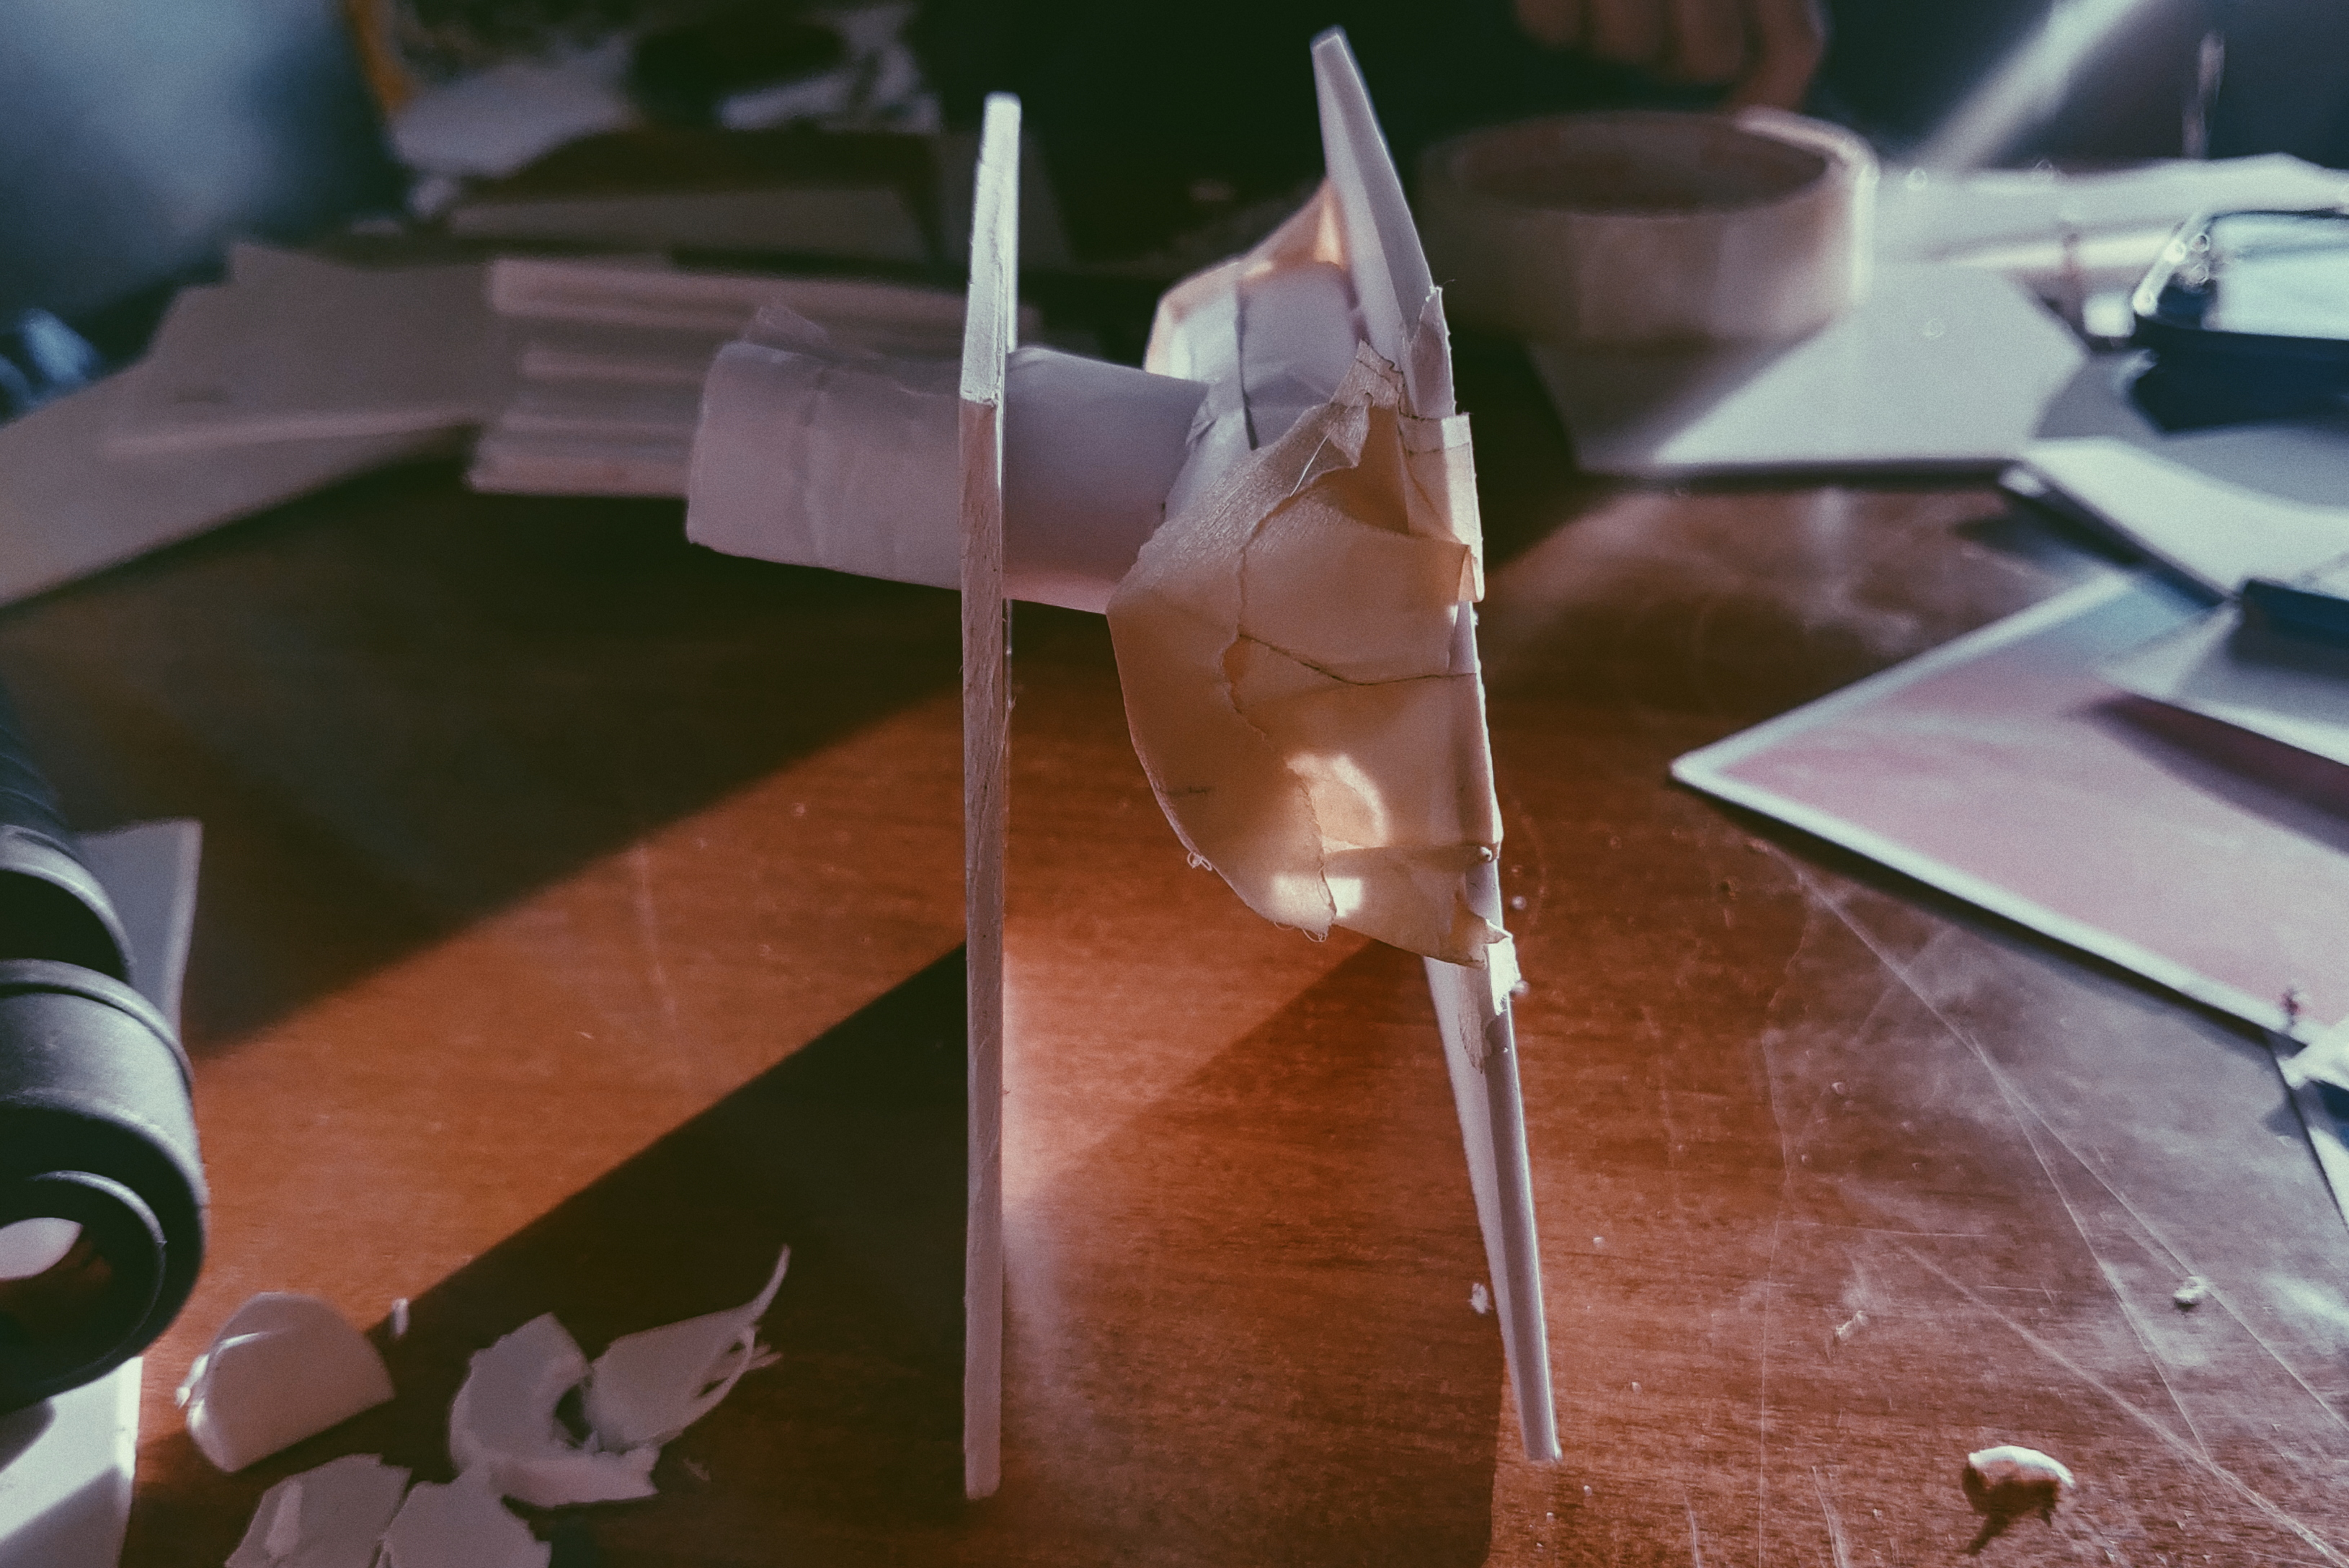
\includegraphics[width=0.7\textwidth]{papertool4.jpg}
\end{figure}

\begin{abstract}
	 This project explores the possibilities of teaching AI to schoolchildren (K-12). We are exploring its relevance in K-12 education space — including questions like if we need teaching about AI in K-12 and if it is, what are some meaningful ways to incorporate AI in the existing school curriculum. In a conscious attempt to present a neutral standpoint and accessible method, a paper-based teaching-toolkit is proposed to have open-ended participation from all children. This experimental toolkit intends to break down the complexities of AI, using concepts such as order and chaos, understanding patterns, ethics, and biases. Introducing visual/graphical mathematics could bring in clarity of understanding both mechanisms and behavior, and a sentient acceptance of patterns and models. Given multiple interpretations of intelligence, this intervention will also enable children to define it themselves subjective to their analysis.
\end{abstract}

\begin{figure}[h]
  \center
  
\includegraphics[width=\textwidth]{sigmoid_roadmap.png}
  \caption{Project Roadmap}
\end{figure}

\section{Situation}
Situation
With the steady development in the field of AI over the several last decades, and in particular, the recent interest in AI-driven business use cases and its penetration across the computing and technology-driven spaces \cite{Anexecut56:online}, it is increasingly becoming relevant for professionals in such areas to be aware and proficient in AI. 

There is an emergence of AI-related courses and programs at undergraduate and above levels of study. In schools, however, its perception is limited to mathematics and science. The National Achievement Survey (NAS) 2018 found that Indian school children lose grip on math and science as they enter higher classes. \cite{educatio96:online} Empirically it can be seen that this lack of interest in mathematics and science is because of a lack of relating to the context or finding relevance in what is being talked about. As a result, active thinking is about this is not encouraged and as a result, there is very less participation or contribution. This can be addressed by providing probes at points where children seem to deviate interest, where they begin to lose grip of their chain of thought, and provide opportunities to express and mould their understanding physically.

Artificial Intelligence as a subject is only offered at undergrad or higher levels.  And students then identify or told that the domain requires good understanding of mathematics and programming. But why or how would something as broad as intelligence be limited to a single field of study? Through this study, we may be able to find ways to integrate all fields to intervene and bring up the ethical AI of the future.

While the relevance of AI systems is more apparent in urban areas that can afford and utilise technology first-hand, 66\% of India’s population comes from the rural sector. It would be important to make the study accessible and affordable for all sectors. A physical paper toolkit is chosen to have this intervention accessible for everyone. 

\section{Objective}
To explore and realise a series of novel and open resources to teach AI in schools. 

\begin{itemize}
  \item Developing low-cost paper based toolkits to enable teaching AI in schools. 
  \item Developing simple and beginner friendly introduction to AI by scaffolding technical complexity of implementing AI.
  \item Creating artefacts to provoke conversations around AI and ethics in the classrooms 
\end{itemize}

\begin{figure}[h]
  \center
  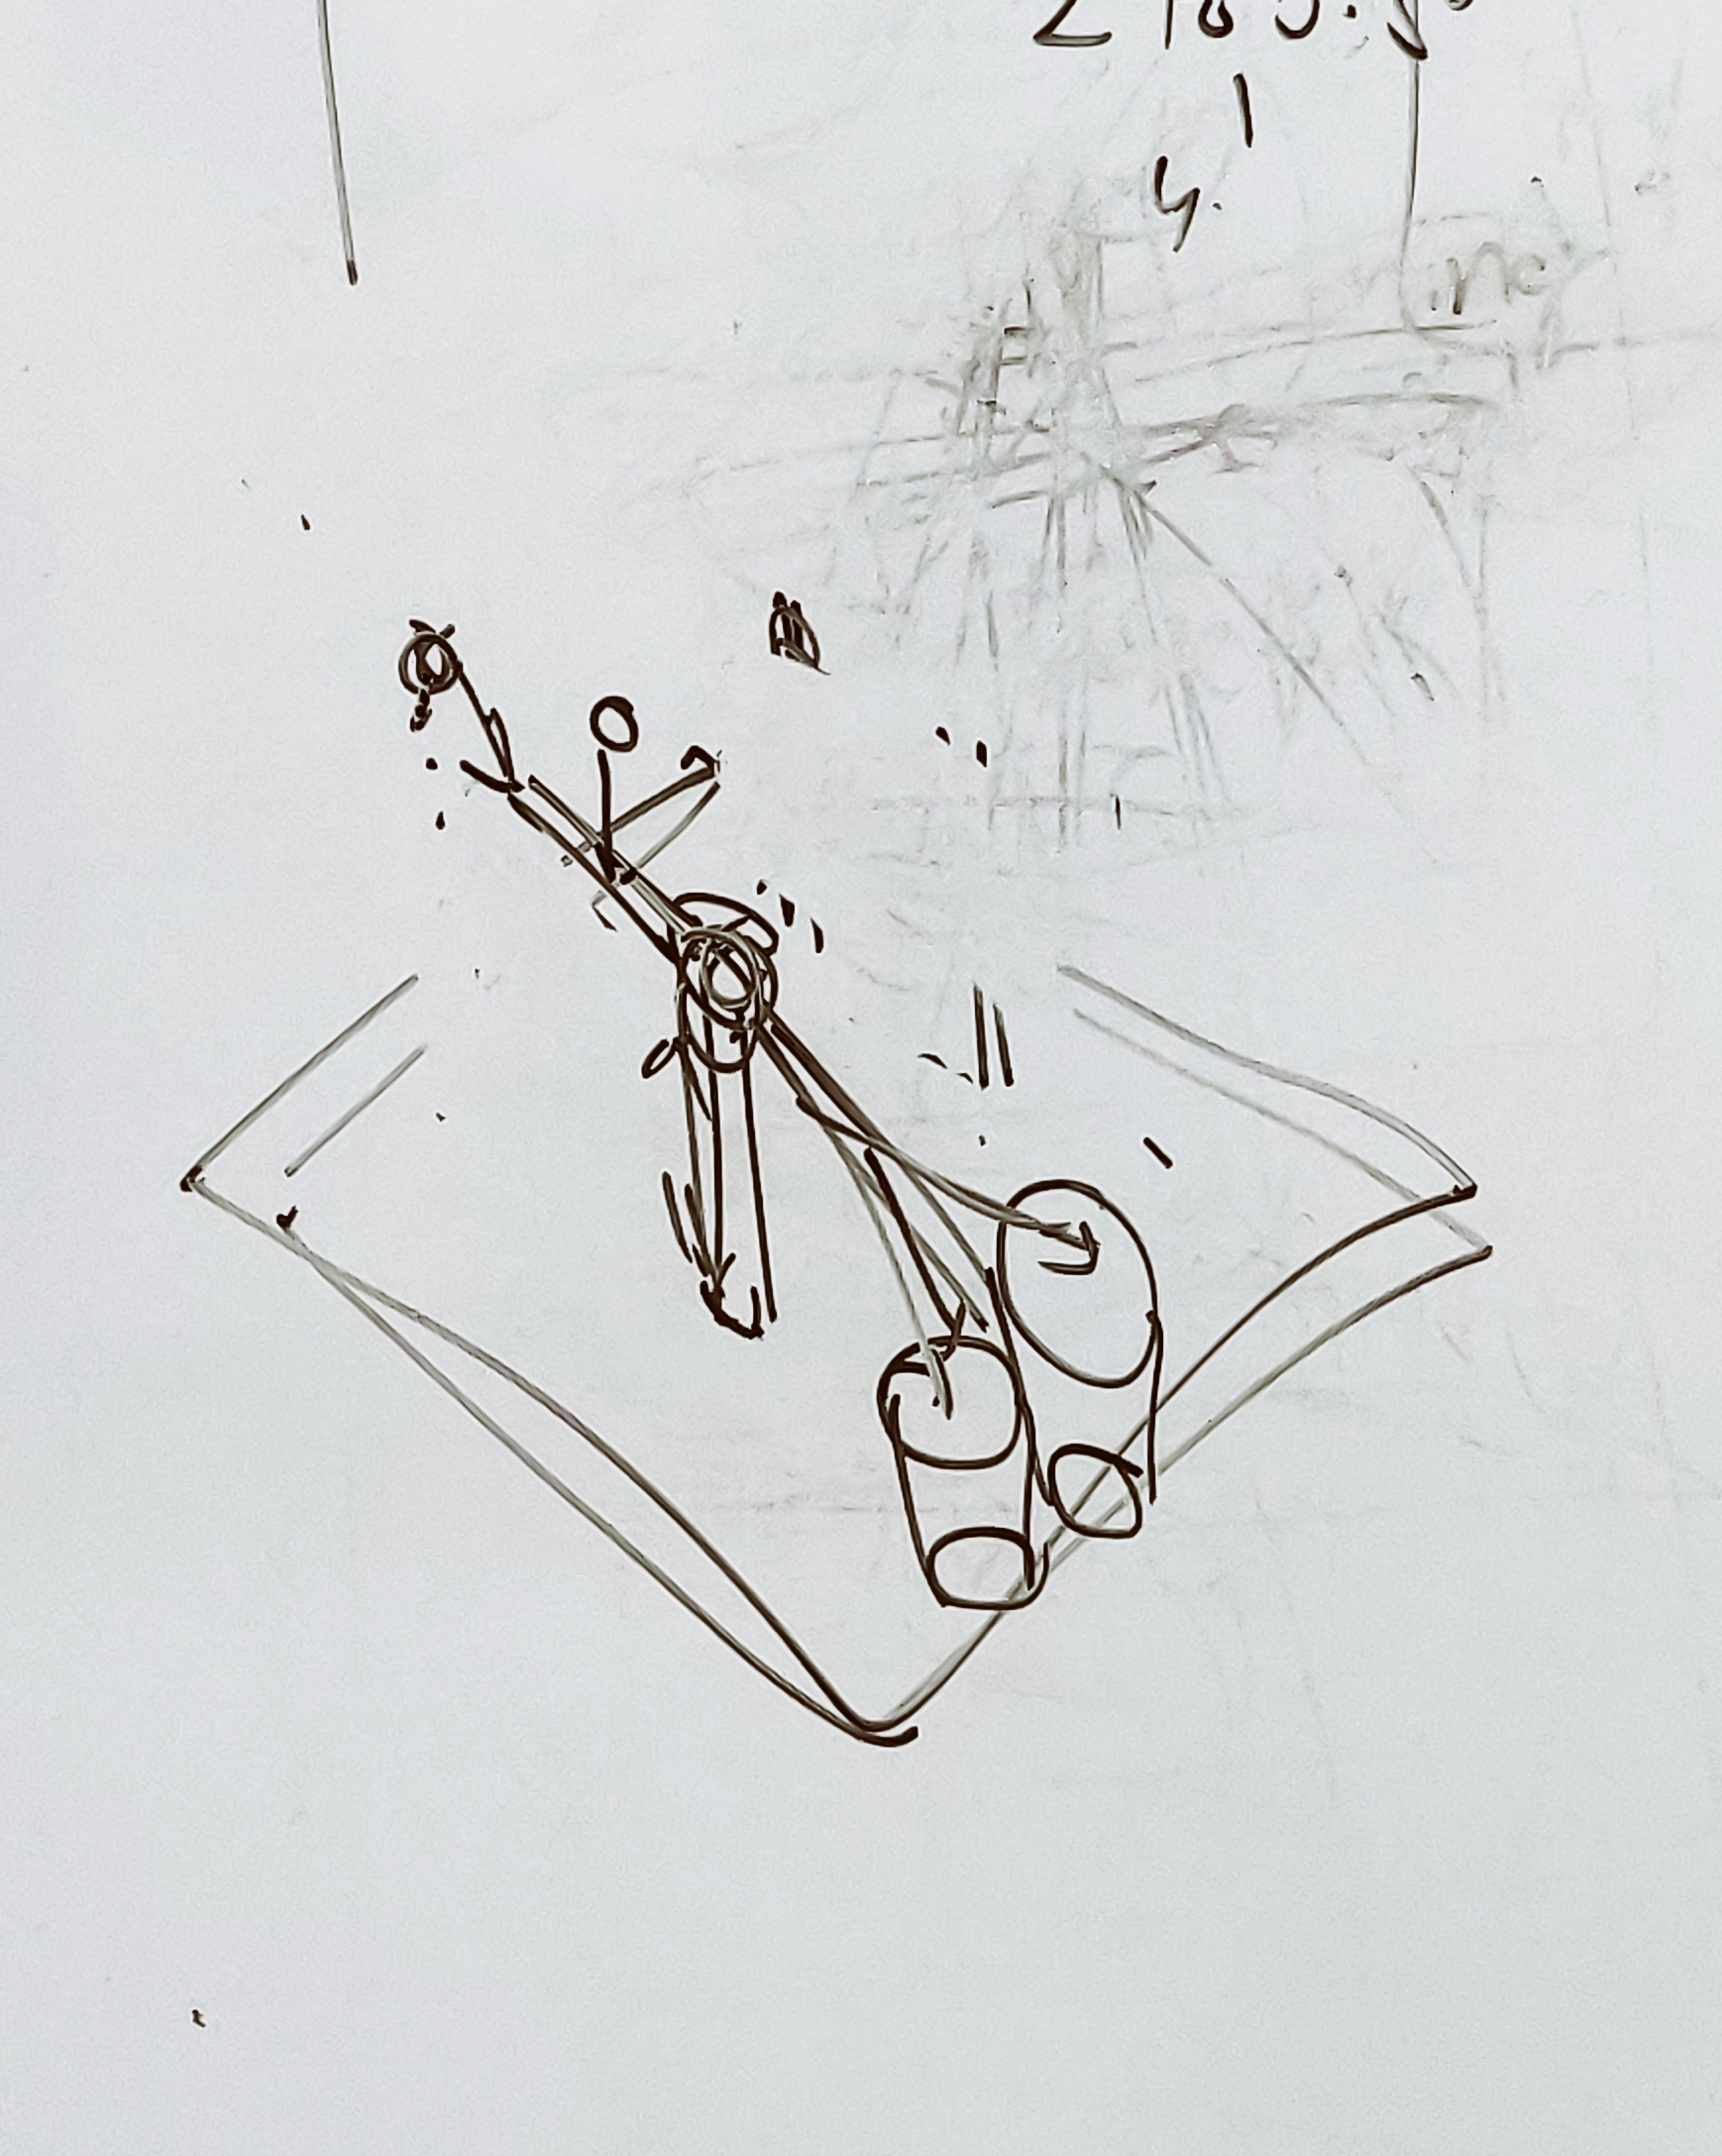
\includegraphics[width=0.4\textwidth]{papertool1.jpg}
  \caption{Imagining paper prototype of perceptron}
\end{figure}

\section{Approach}

\begin{figure}[h]
  \center
  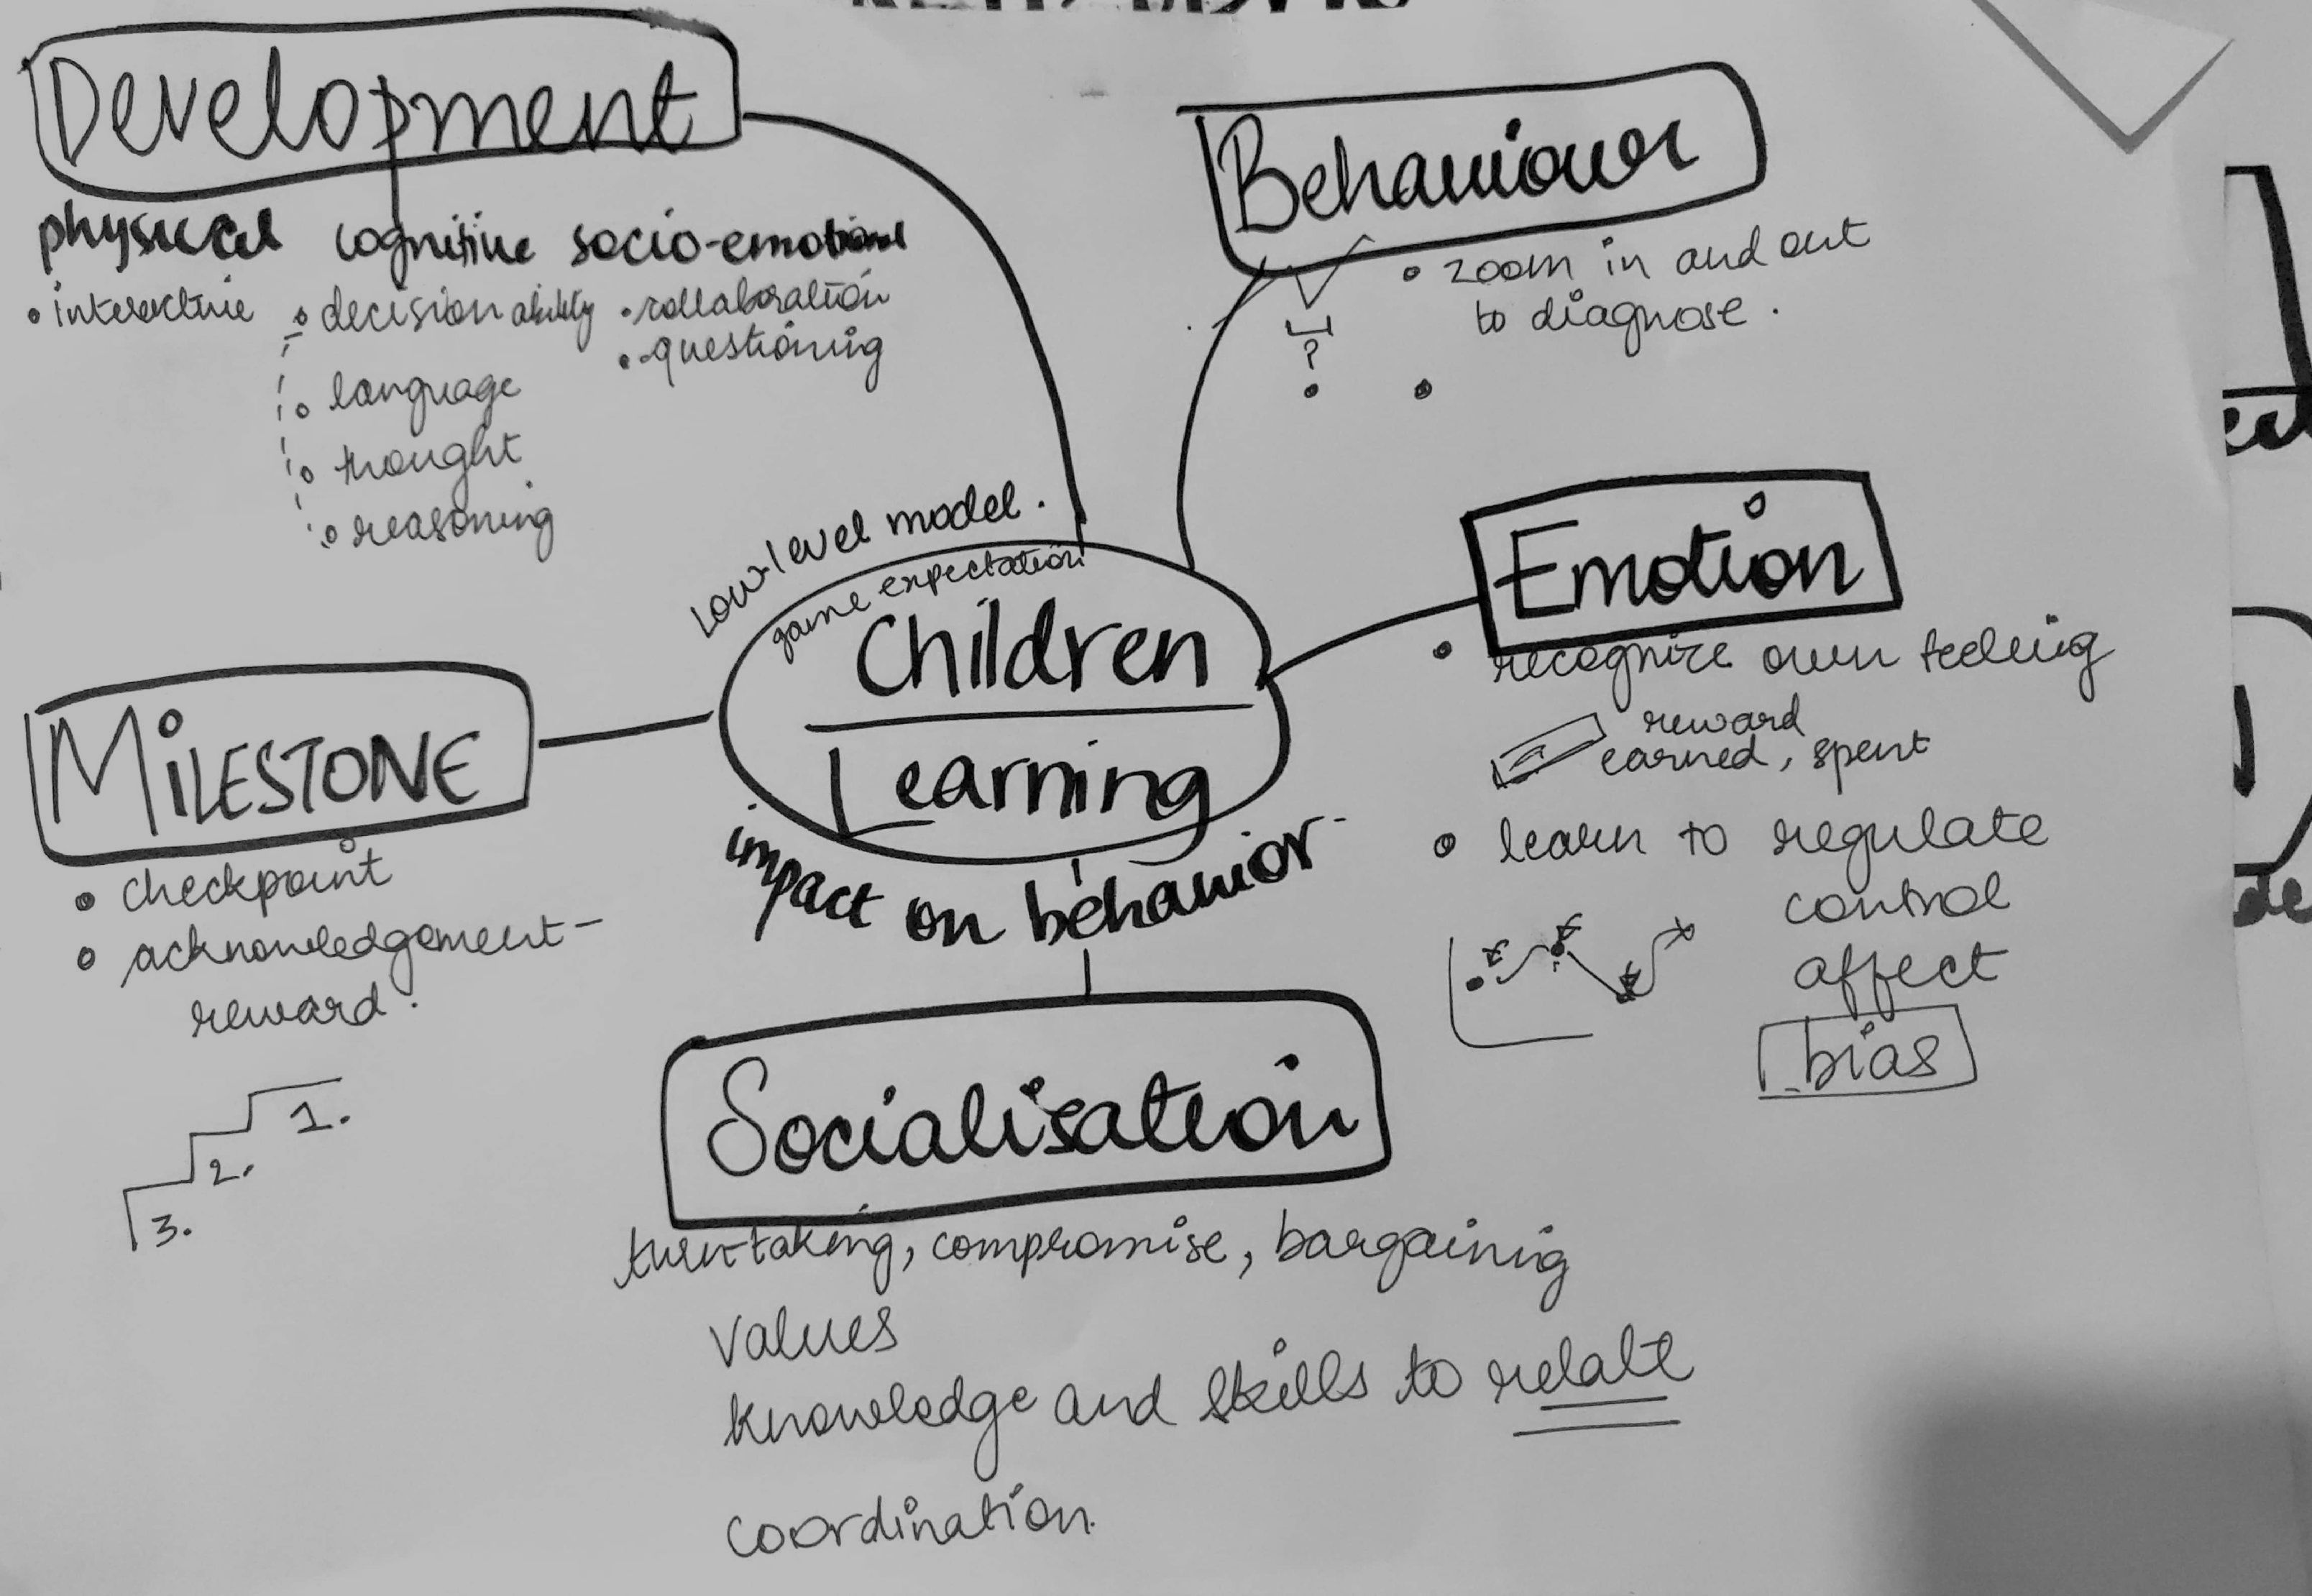
\includegraphics[height=0.25\textwidth]{block1-1.jpg}
  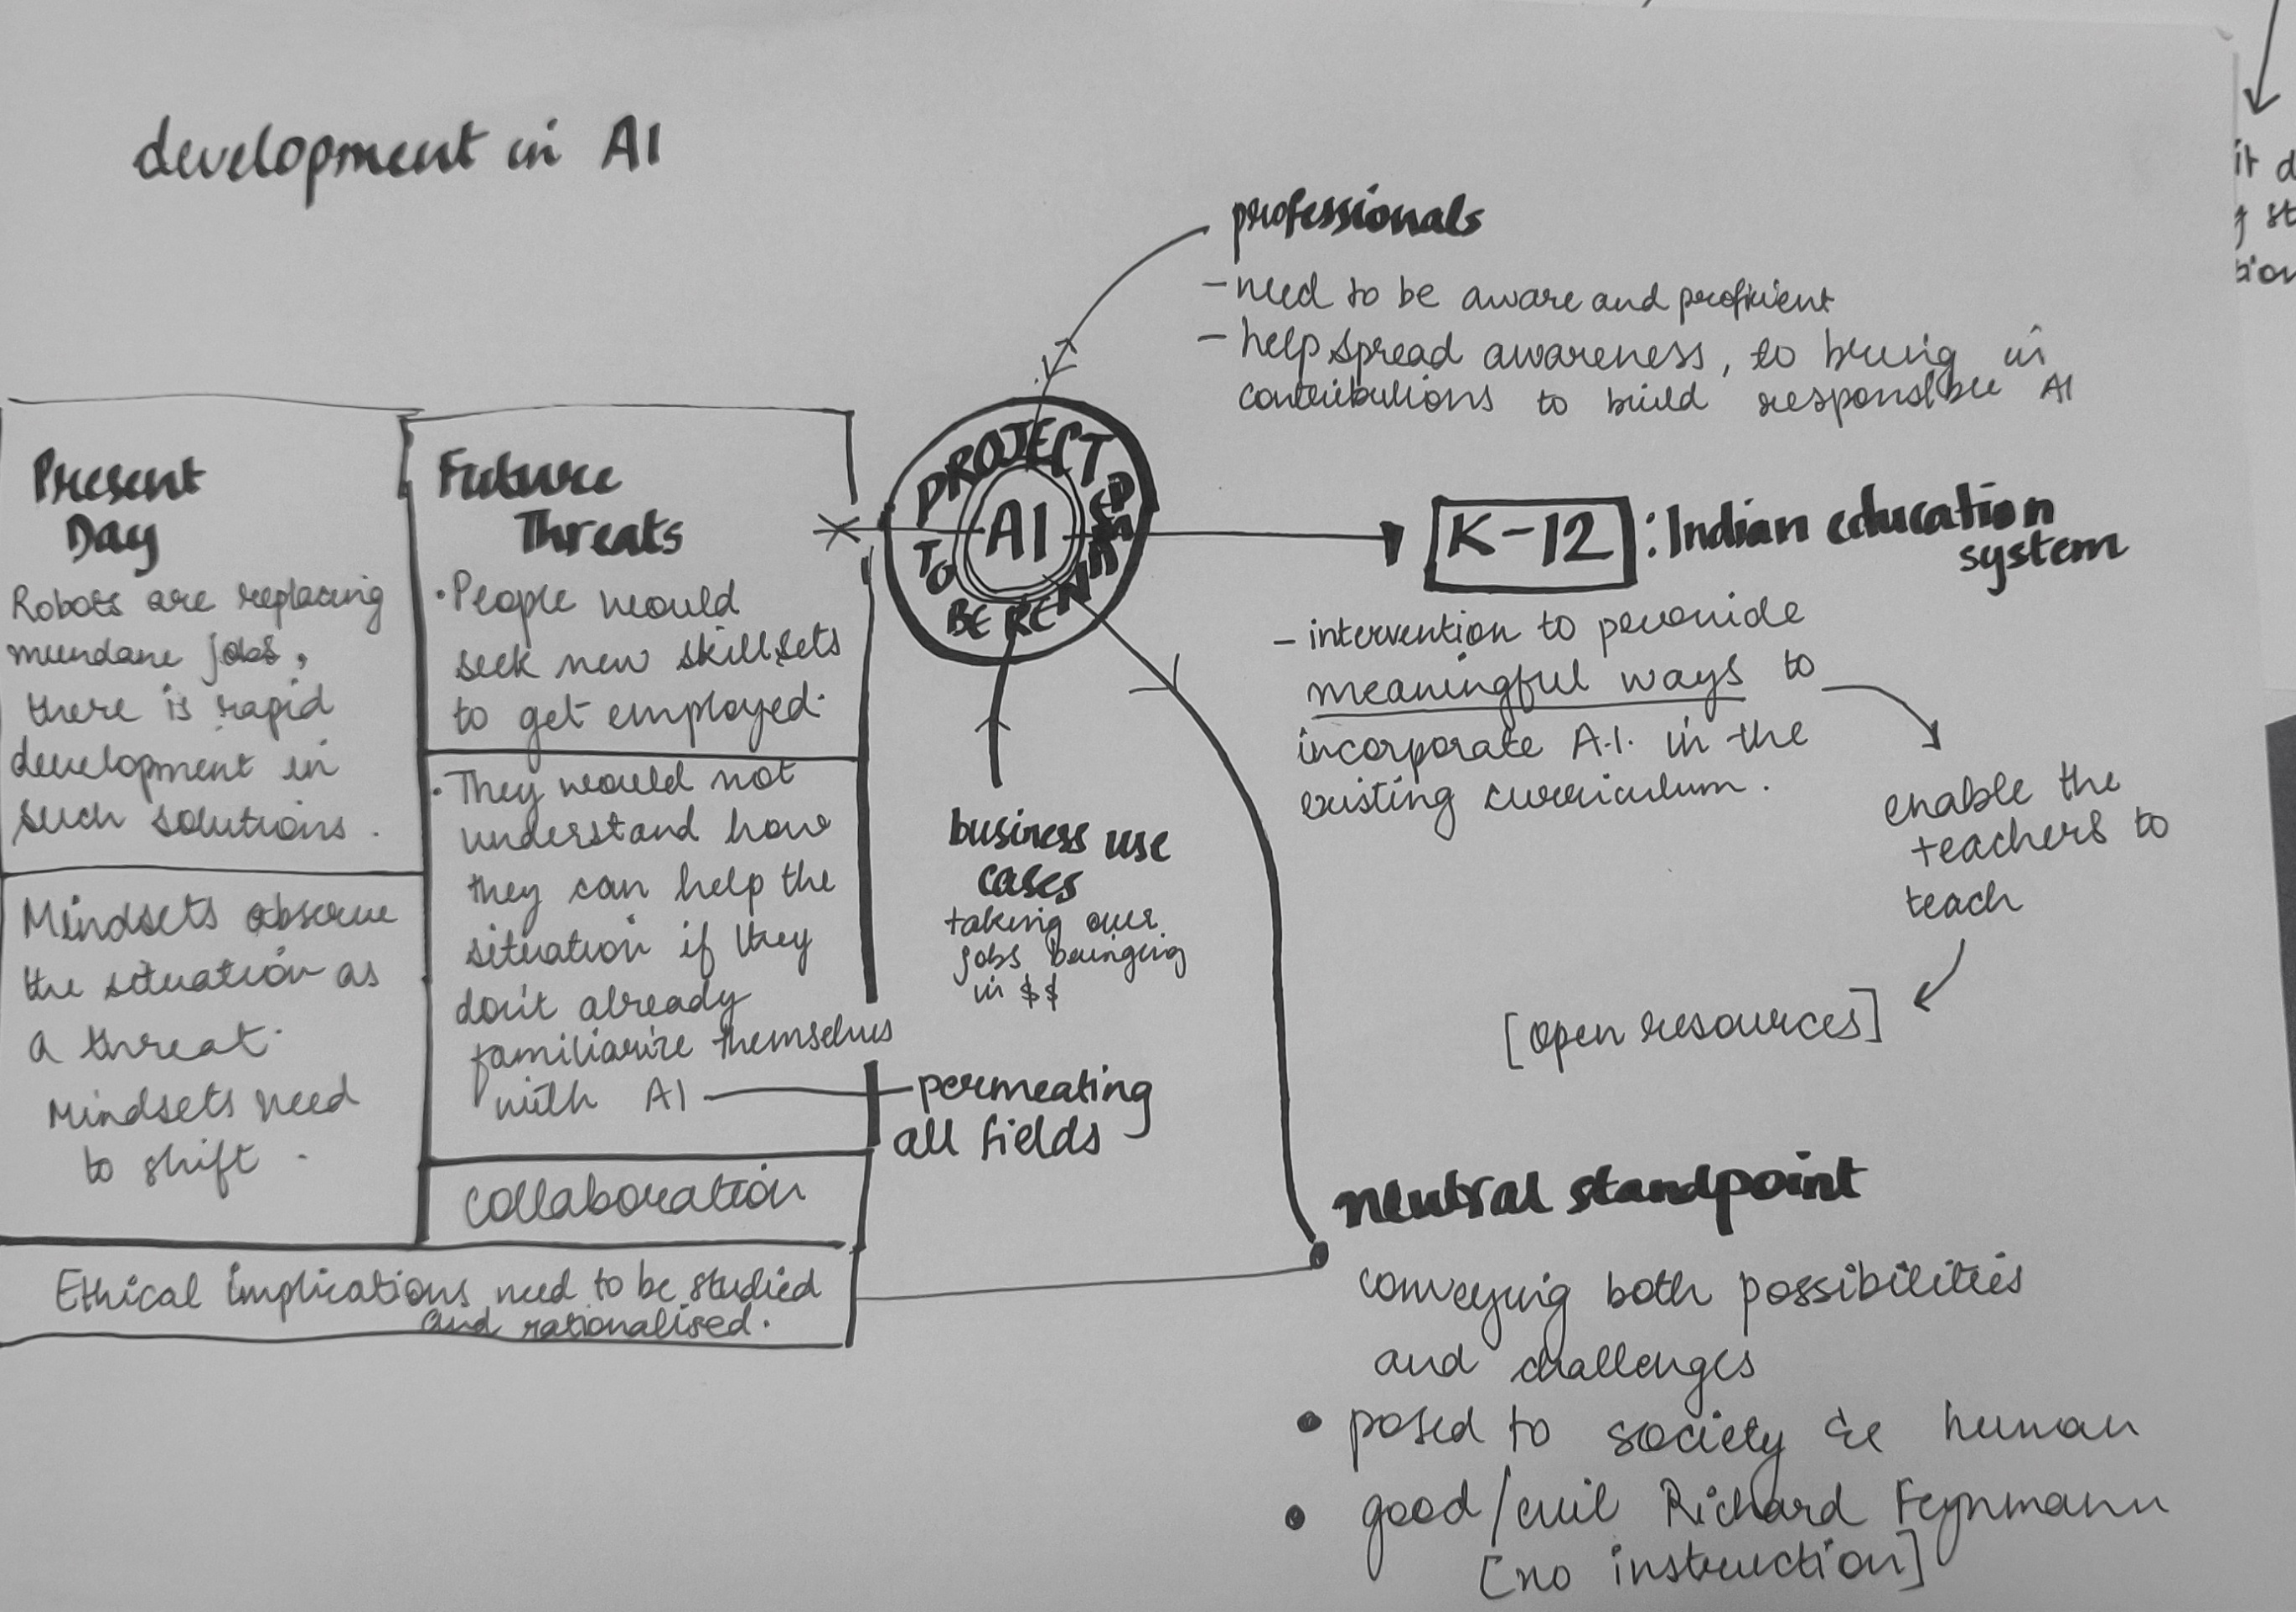
\includegraphics[height=0.25\textwidth]{block1-2.jpg}
  \caption{Initial mapping}
\end{figure}

\textit{How might we teach children about AI through a physical toolkit?}

The experts have learnt AI through extensive reading, programming and mathematical affinity with rigorous practice. Our target audience, children should not be overwhelmed with information the same way. To break down these vast diverging concepts into simpler, engaging interactions, we first decided to look into machine learning as a subset of AI At many points, learning in children was compared to machine learning, drawing parallels in everyday life (example: making a cheese sandwich) step by step approach to understand algorithms.

$$ y = w.x + b $$

\begin{figure}[h]
  \center
  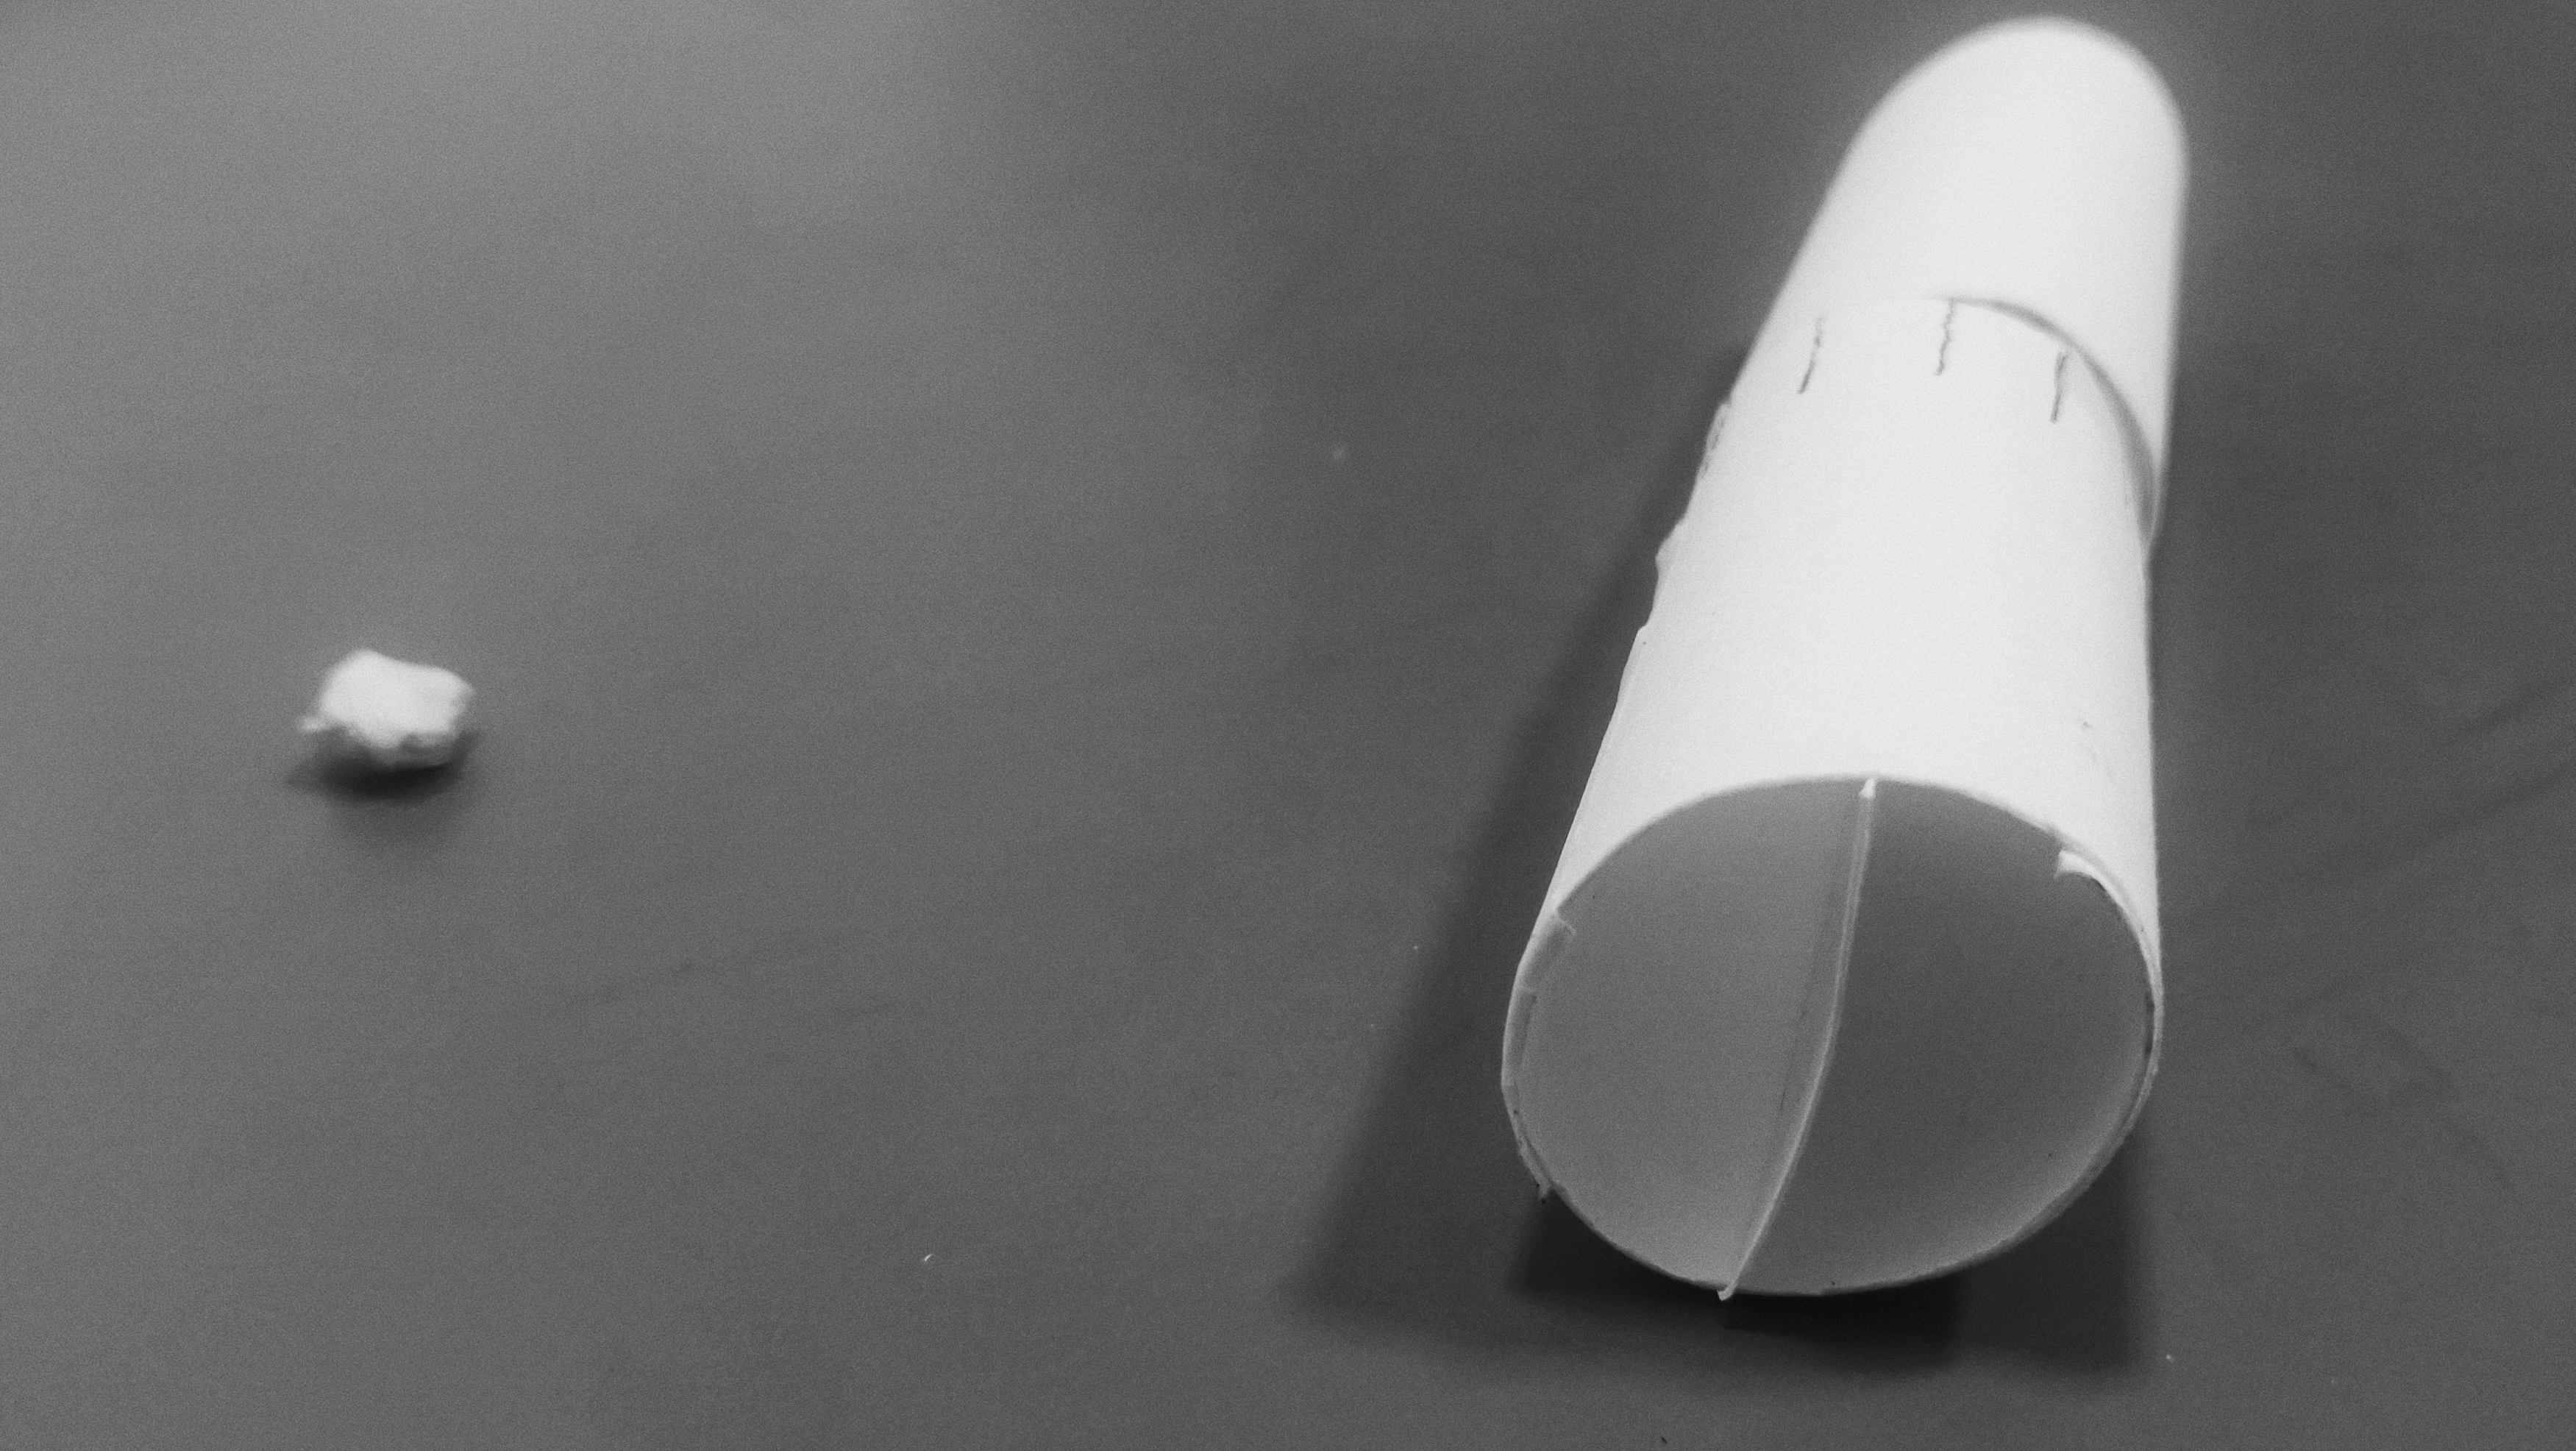
\includegraphics[width=0.4\textwidth]{papertool2.jpg}
  \caption{Paper prototype of the perceptron}
\end{figure}

A simple input/output machine process using a paper ball as data and pipes as the network with weight fluctuation and adjustment was explored. 

The lower side of the input pipe would rotate in order to set the weight. The output pipe would be adjusted according to the weight to show different outputs. The functionality of every part of a neuron is translated in this idea. A few more related forms with varying materials (magnets, slides, height) were used to show affected input ball inside the pipe as it travels.

\begin{figure}[h]
  \center
  
\includegraphics[height=0.4\textwidth]{papertool5.jpg}
  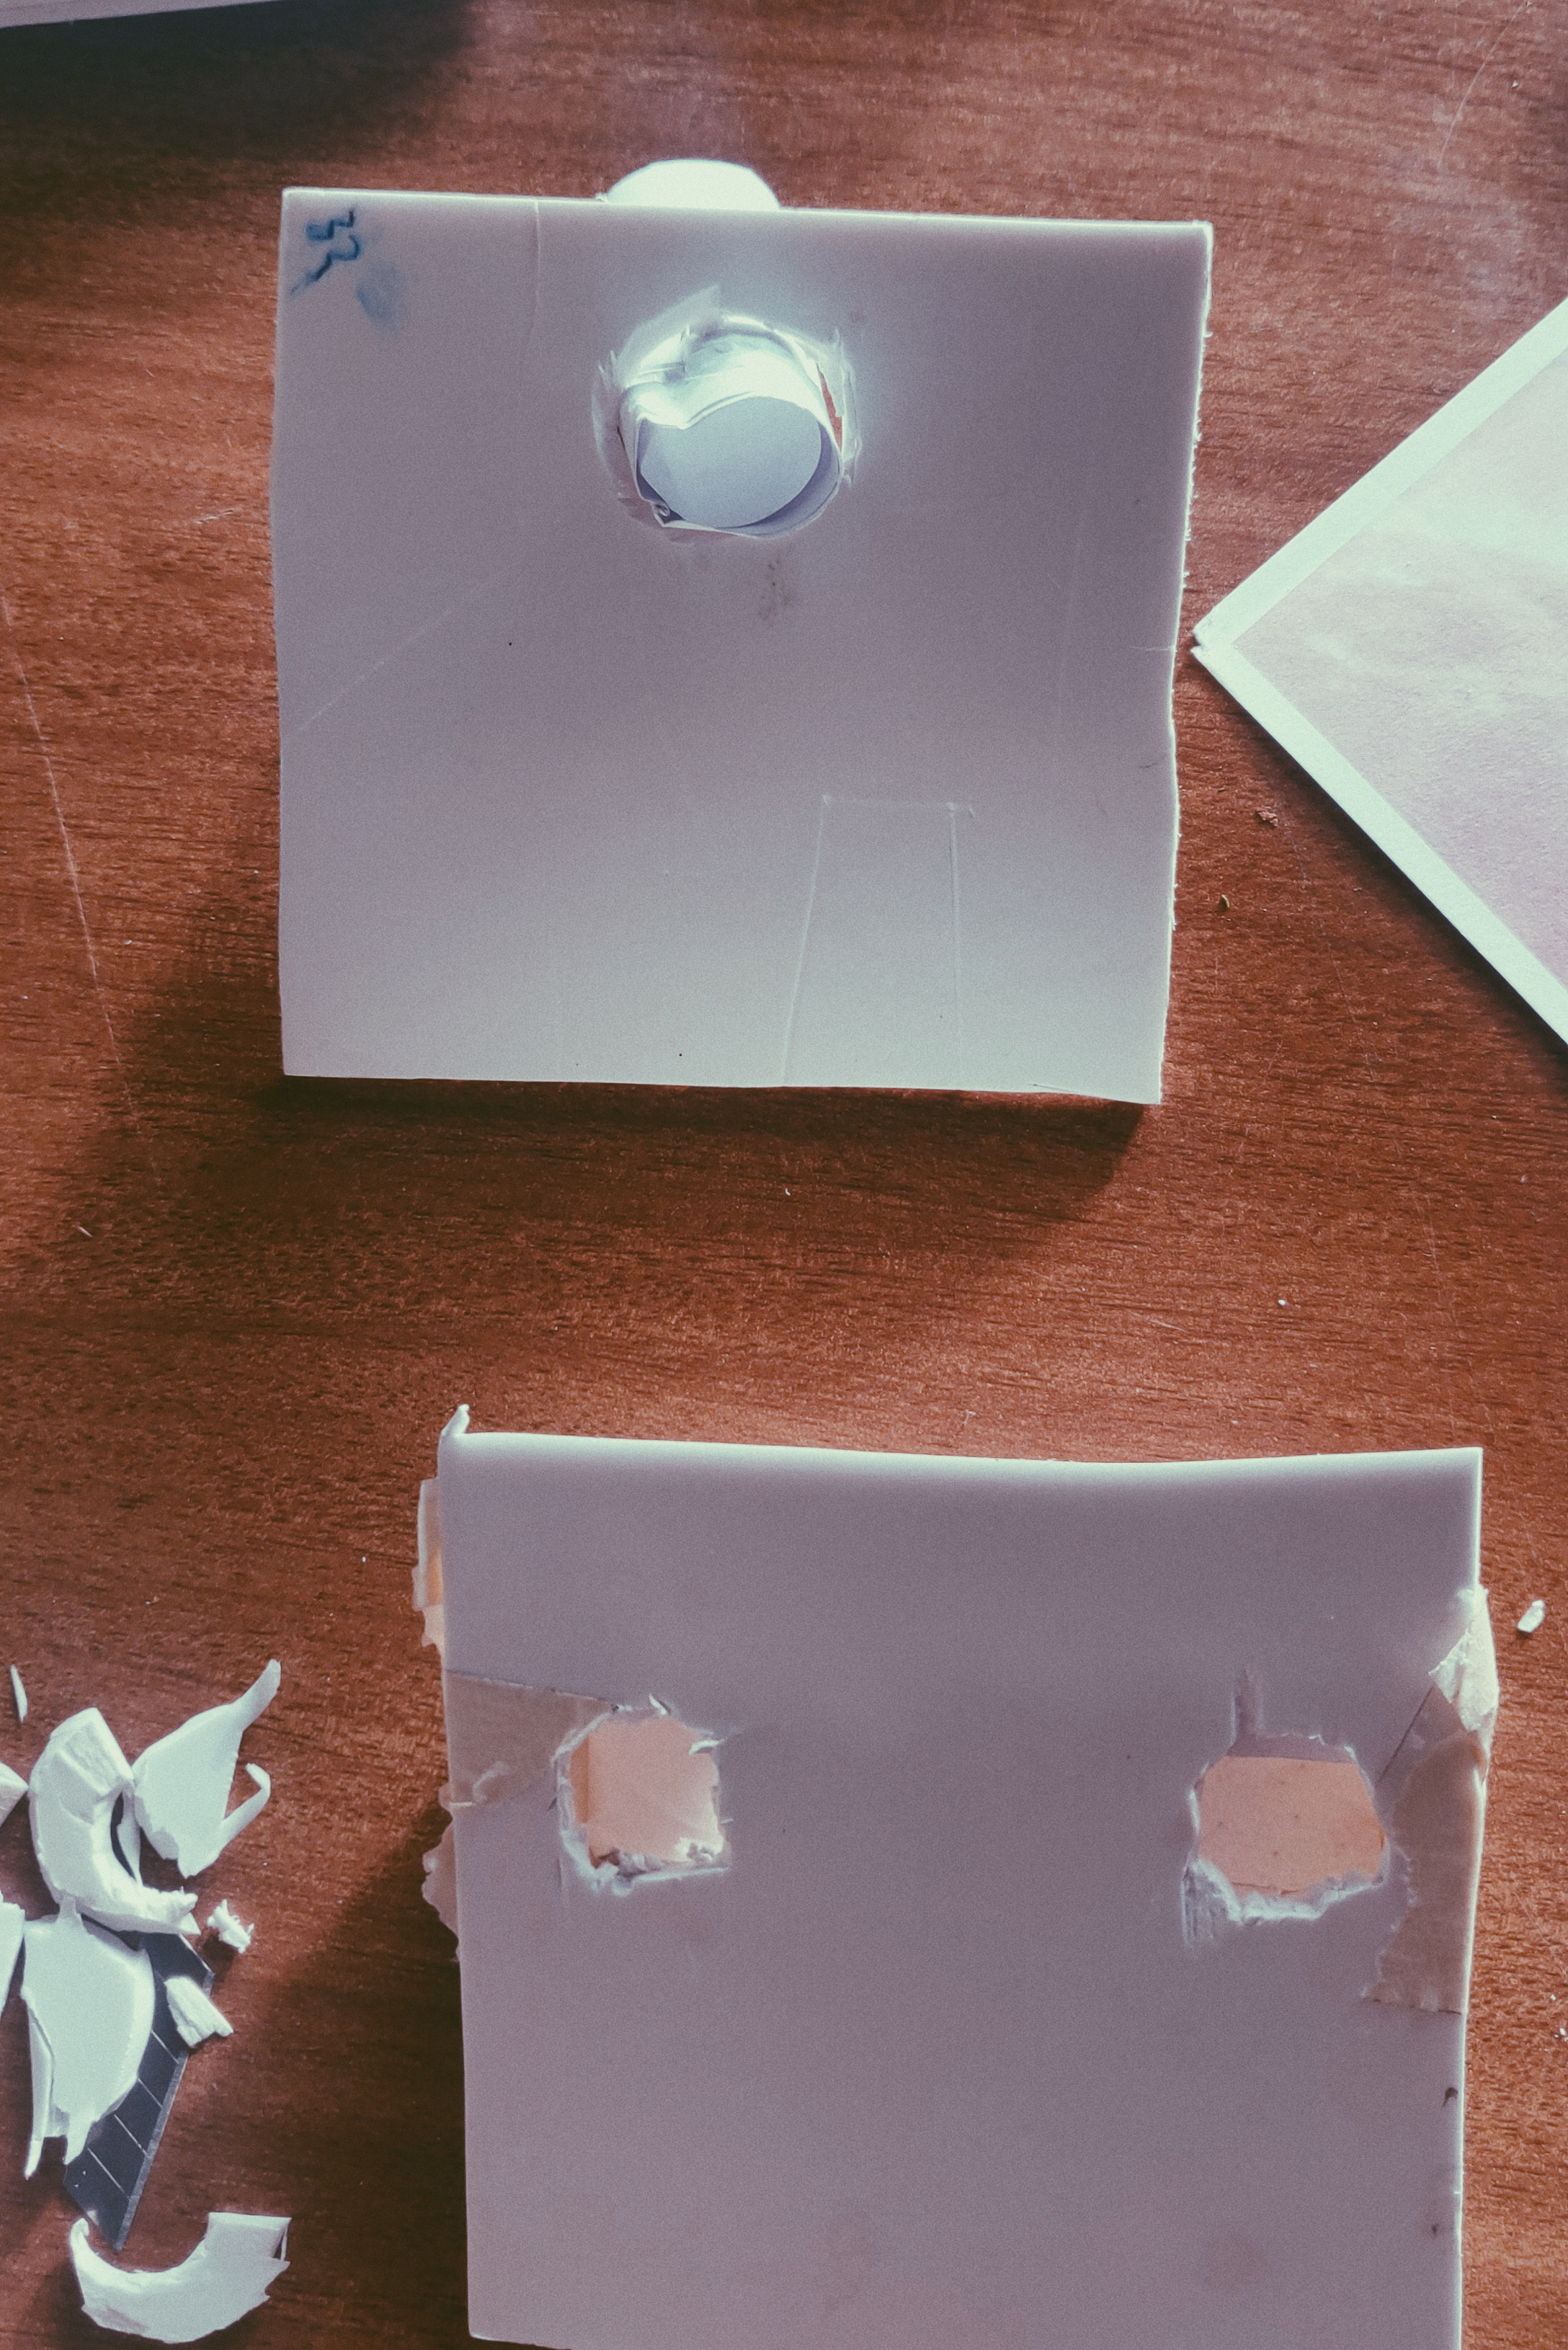
\includegraphics[height=0.4\textwidth]{papertool6.jpg}
  \caption{Blackbox idea -- slides in the blackbox to construct the machine per choice}
\end{figure}

One problem seen in this approach was the need to define every related part and function being performed.  Avoiding them would not be fair, and defining them as they go felt important. But the very fact that one process can’t fathom the definition of intelligence, same as not knowing the one universal machine learning model, started to become a cause for concern. 

Keeping in mind that our perception of intelligence, looking at how we see and comprehend things around us found us further direction. Related concepts and implications would have to be introduced, made simpler yet engaging enough to pursue from start to finish without getting lost on the way. In order to teach Artificial Intelligence to children, intelligence would need to be understood and defined. Artificiality could make better sense afterwards.

Let us consider the following definitions. 

\textbf{What is intelligence?} The Oxford Dictionary defines Intelligence as the ability to acquire and apply knowledge and skills. Synonyms: intellectual/mental capacity, intellect, mind, brain, brains, brainpower, powers of reasoning, judgement, reason, reasoning, understanding, comprehension, acumen, wit, sense, insight, perceptiveness, perception, perspicaciousness, perspicacity, penetration, discernment, sharpness, quickness of mind, quick-wittedness, smartness, canniness, astuteness, intuition, acuity, alertness, cleverness, brilliance, aptness, ability, giftedness, talent; informal: braininess.

\textbf{What does it mean to be artificially intelligent?} Artificial intelligence refers to the simulation of human intelligence in machines that are programmed to think like humans and mimic their actions. 

But how do we decide if a person or thing is intelligent? And what fuels the certainty behind deciding that? Considering the scope of this project, I take that intelligent children can understand intelligent systems. In some manner, if children are aware of how things work, what other factors affect their working (reasoning), and the ability to acknowledge that there is more than meets the eye could be seen intelligently. Moreover, collective and participatory learning with physical objects can bring in confidence and positive self-esteem, for there will be more than just words to express what is meant.

We changed our approach to ideas by trying to see what a computer as a human is really doing — \textbf{decoding coded patterns}. For example, a picture of a landscape to a machine is a matrix of colored pixels. Humans on the other hand can tell you exactly what it is at a glance. A machine would have to look for patterns in color, spacing and know the pattern for this particular landscape to understand it. What if there was a way of bridging these different approaches to understanding?

\begin{figure}[h]
  \center
  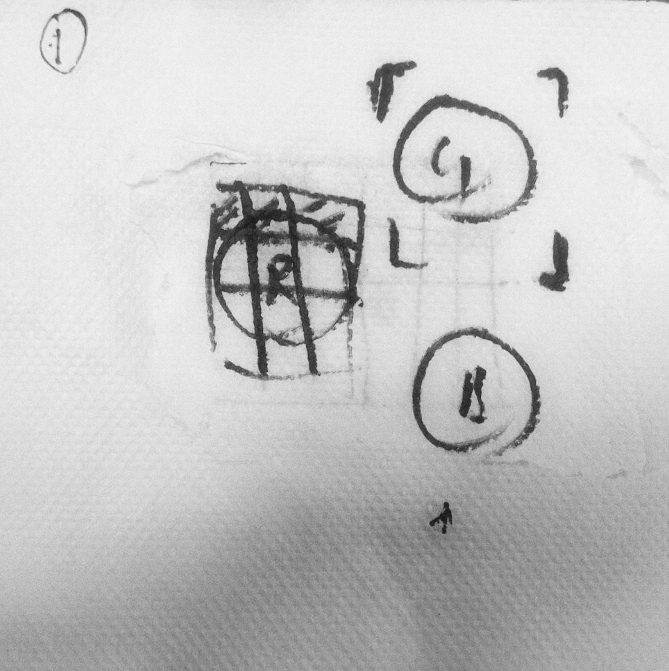
\includegraphics[height=0.3\textwidth]{napkin1.jpg}
  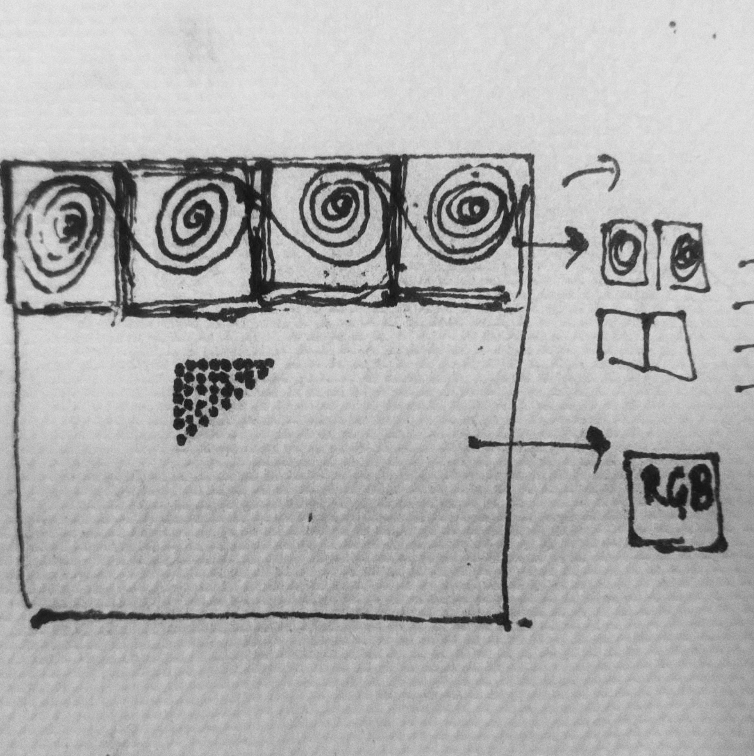
\includegraphics[height=0.3\textwidth]{napkin2.jpg}
  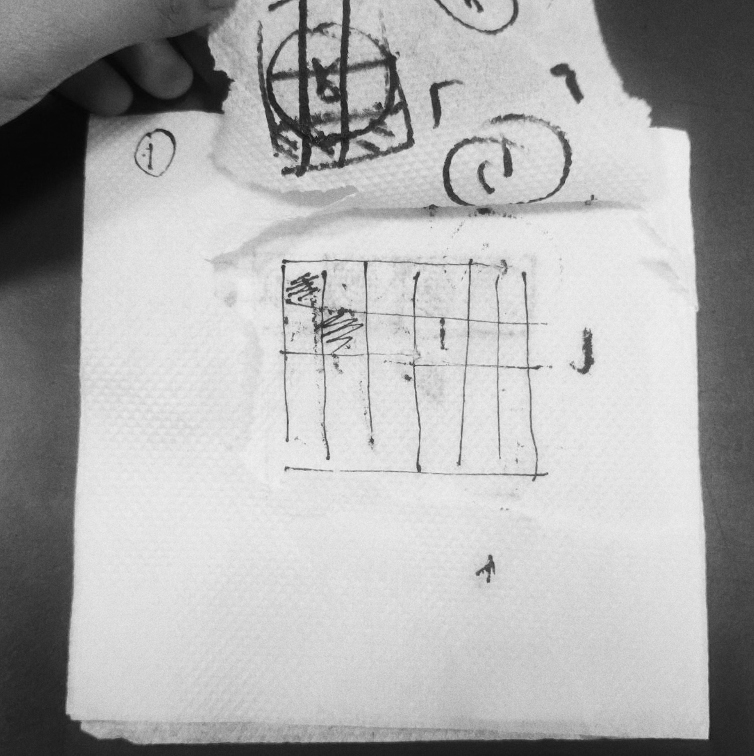
\includegraphics[height=0.3\textwidth]{napkin3.jpg}
  \caption{The napkin idea -- gave way to exploring patterns with the lens of order and chaos}
\end{figure}

Through this exploration, it was evident that both physically and metaphorically, layers hold importance in revealing a sense of priority to create understanding. Order meets chaos as more layers are defined to bridge the between and translate processes intuitively to children. This would also mean less hindrances of big words restricting the journey. This idea was further explored as a paper layered high-low level translation in the toolkit. 

At this point, we were coming across too many ideas that essentially were probing children to think beyond what is apparent. There seems to be no reason to not include an idea since every thought pattern should be valued. However, the lack of a structure could bring in more confusion than we think. I began mapping out elements from every little idea I had in order to group things into categories. While these categories may be overlapping, their presence in a level-up way could be incentivised for active participation.

\begin{figure}[h]
  \center
  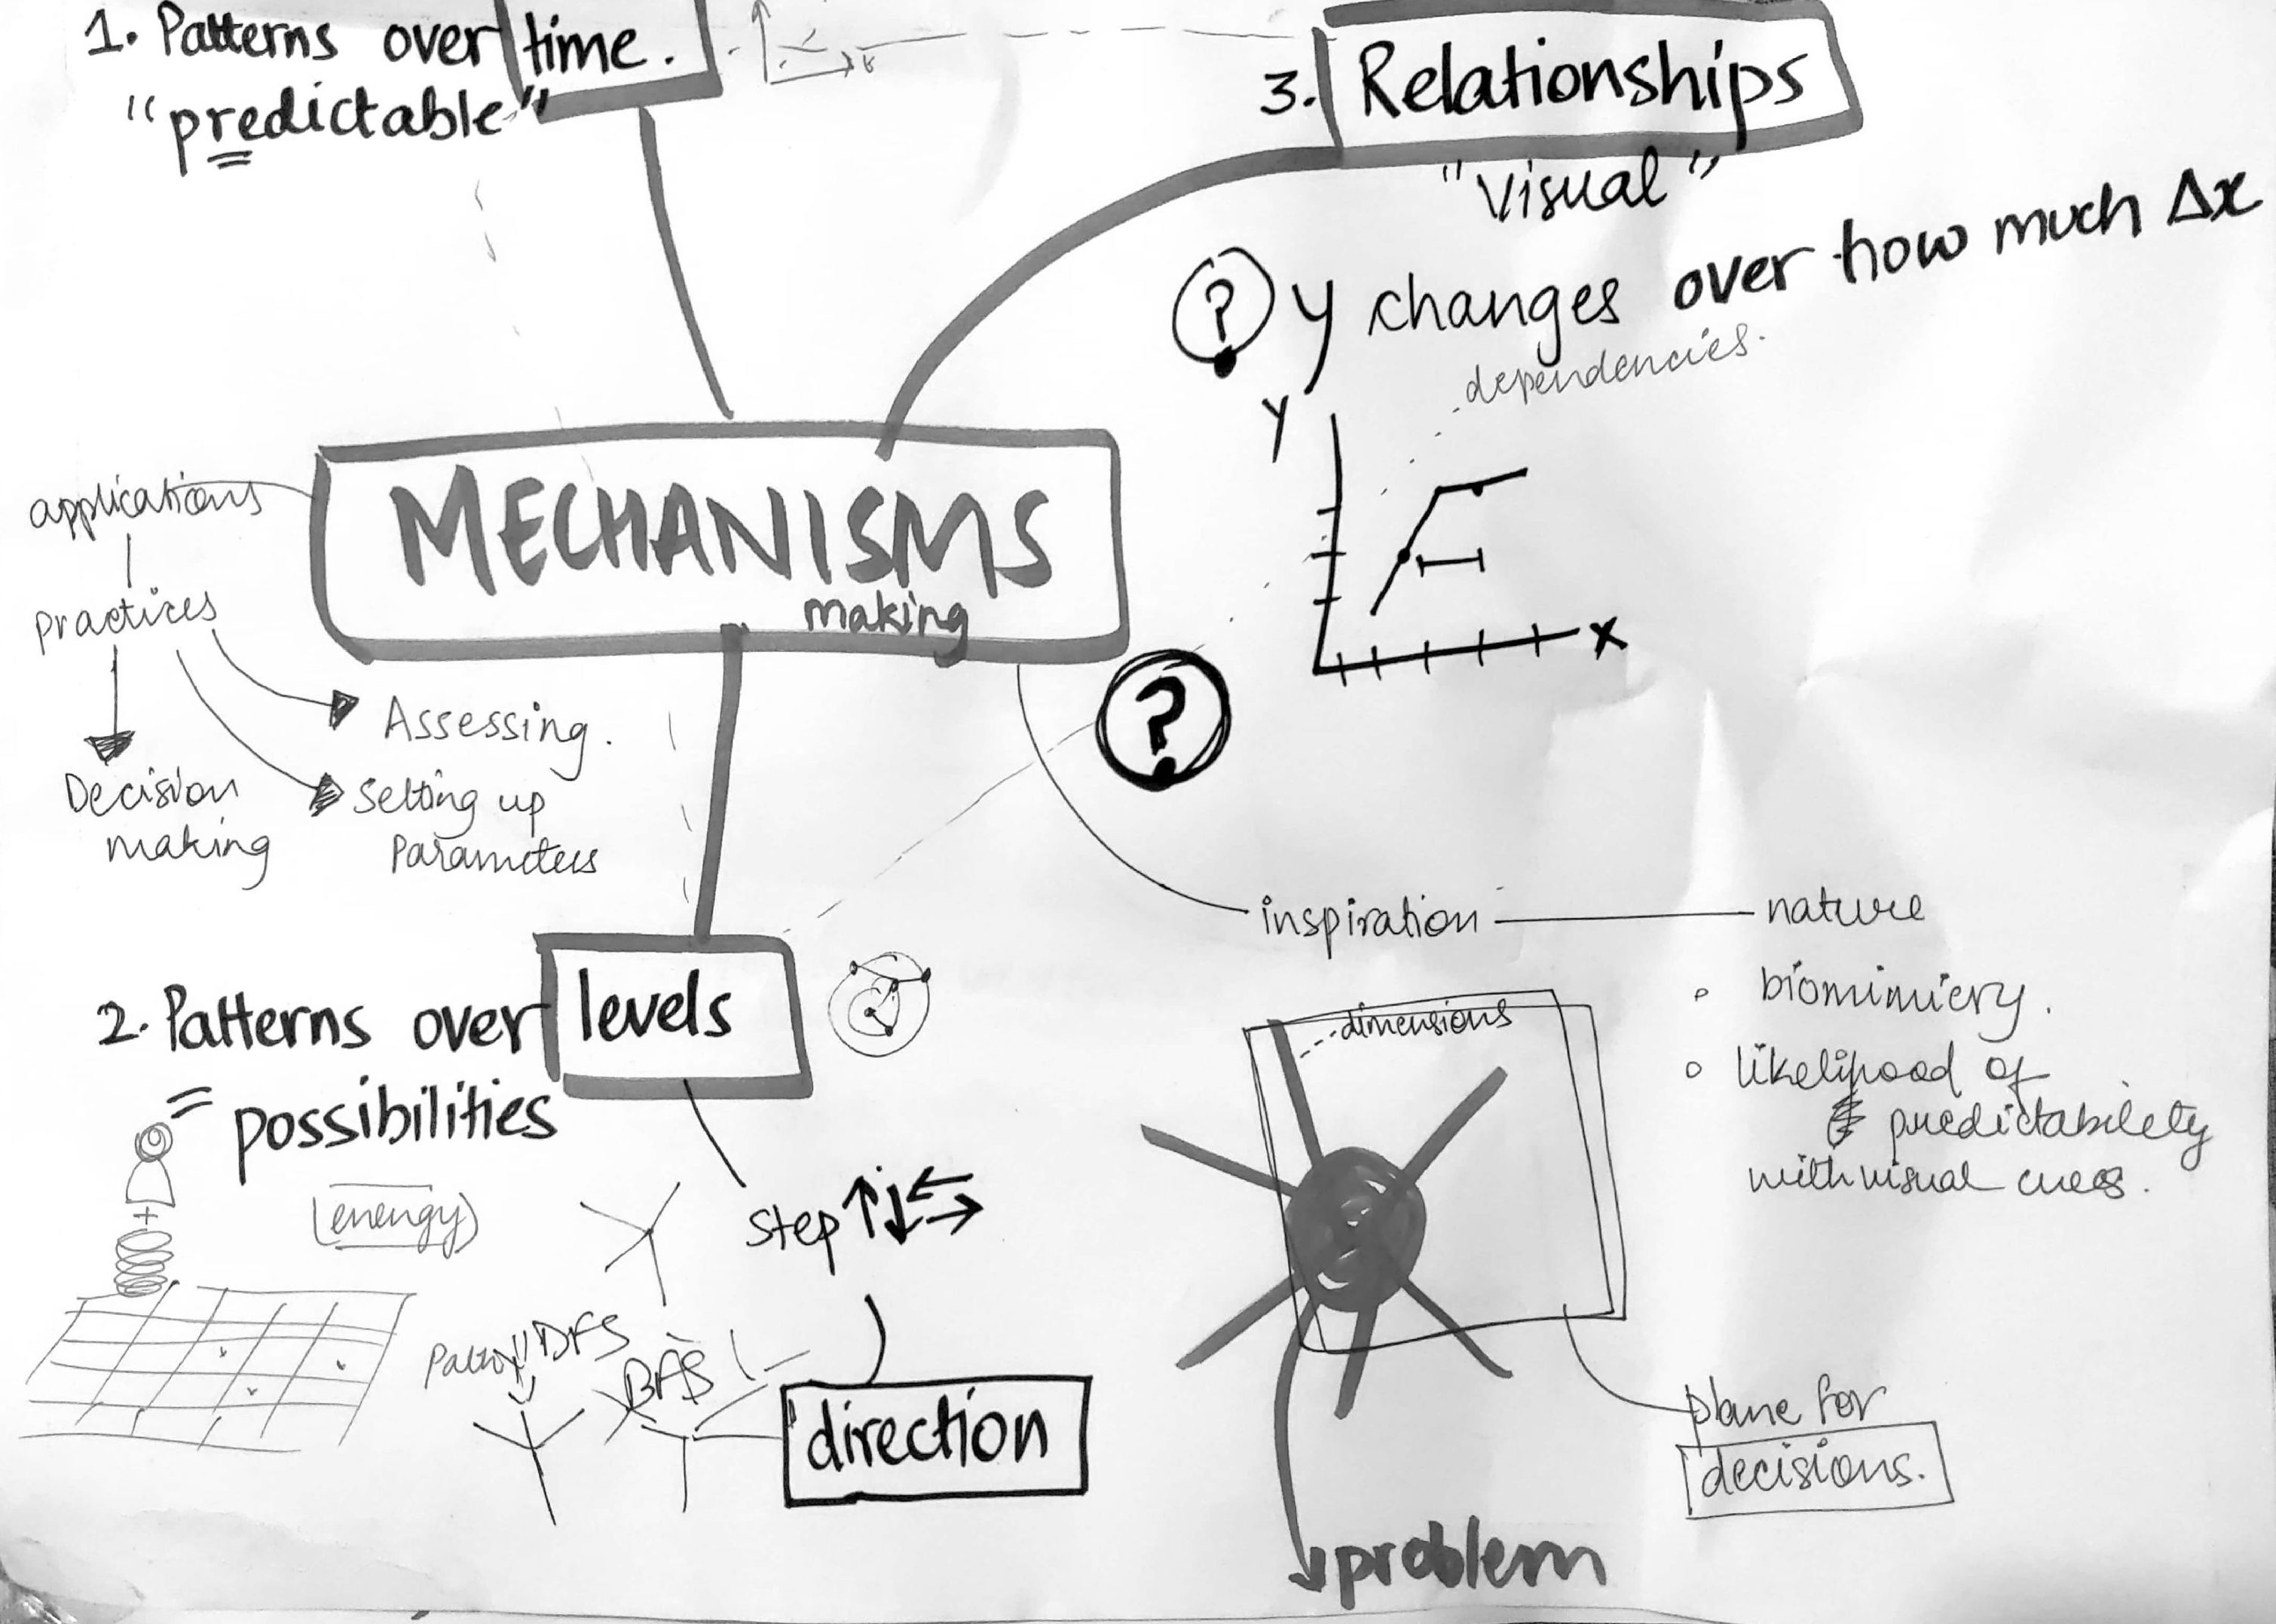
\includegraphics[height=0.2\textwidth]{block6-1.jpg}
  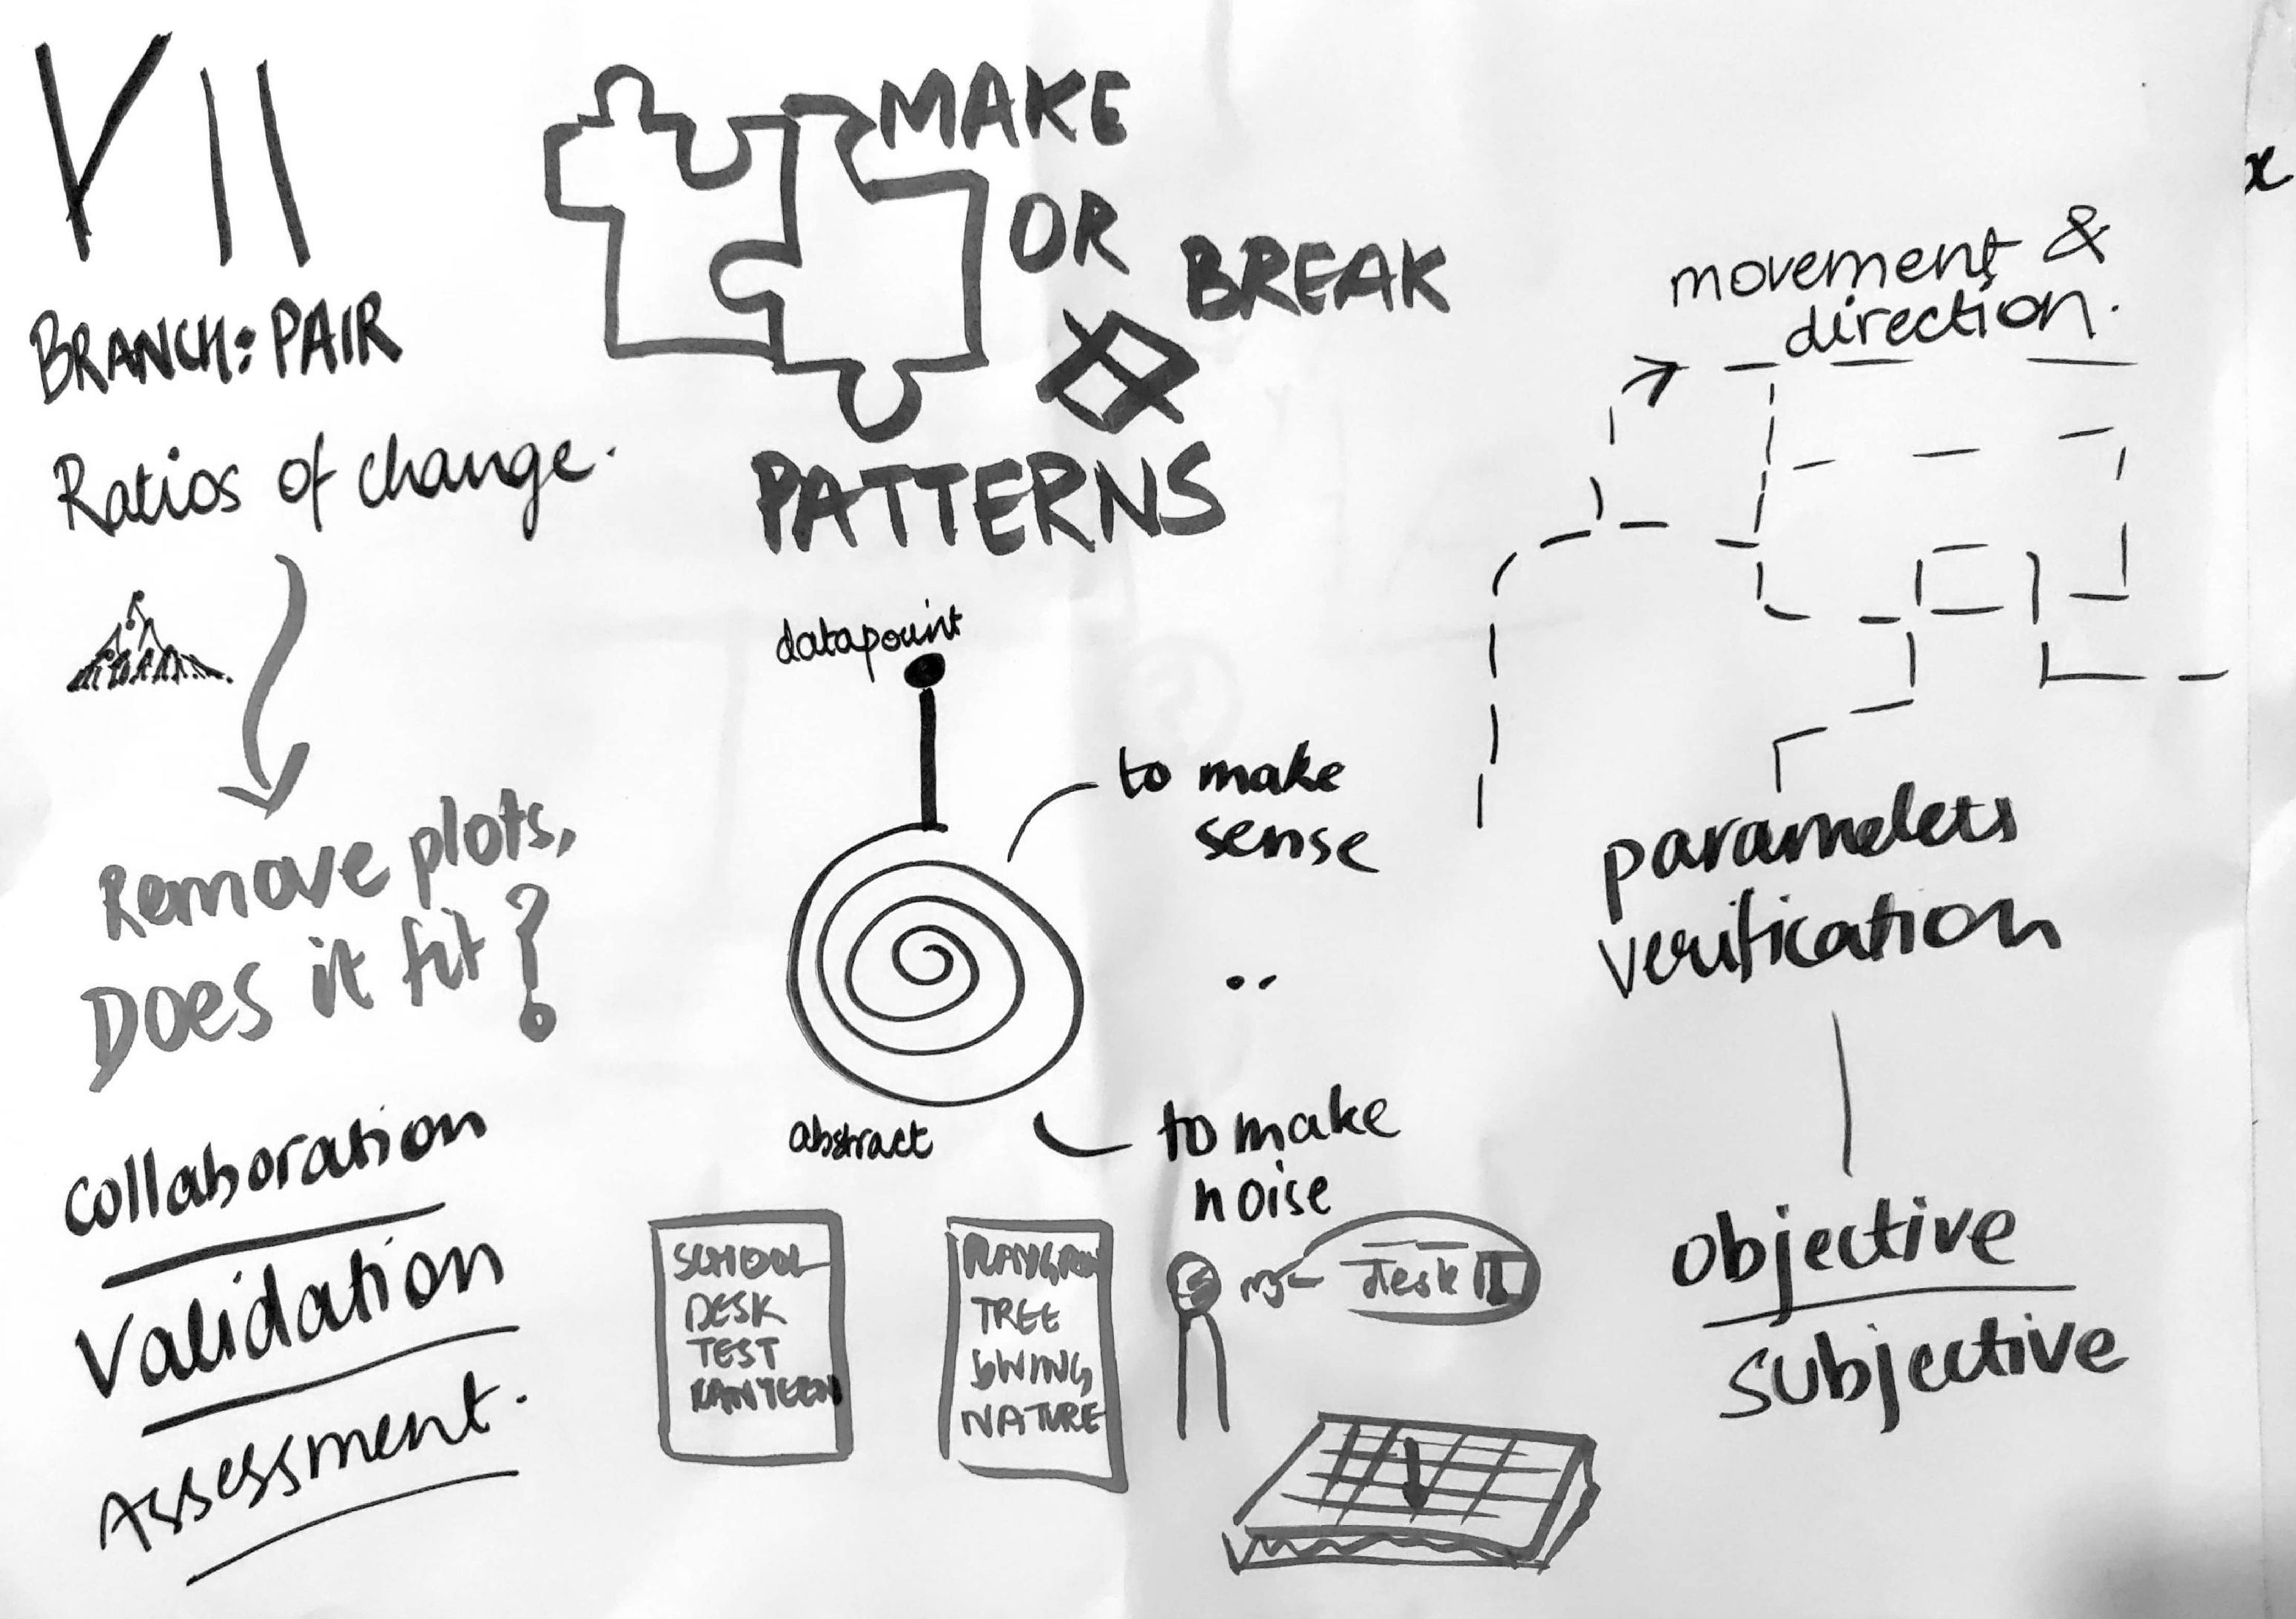
\includegraphics[height=0.2\textwidth]{block6-2.jpg}
  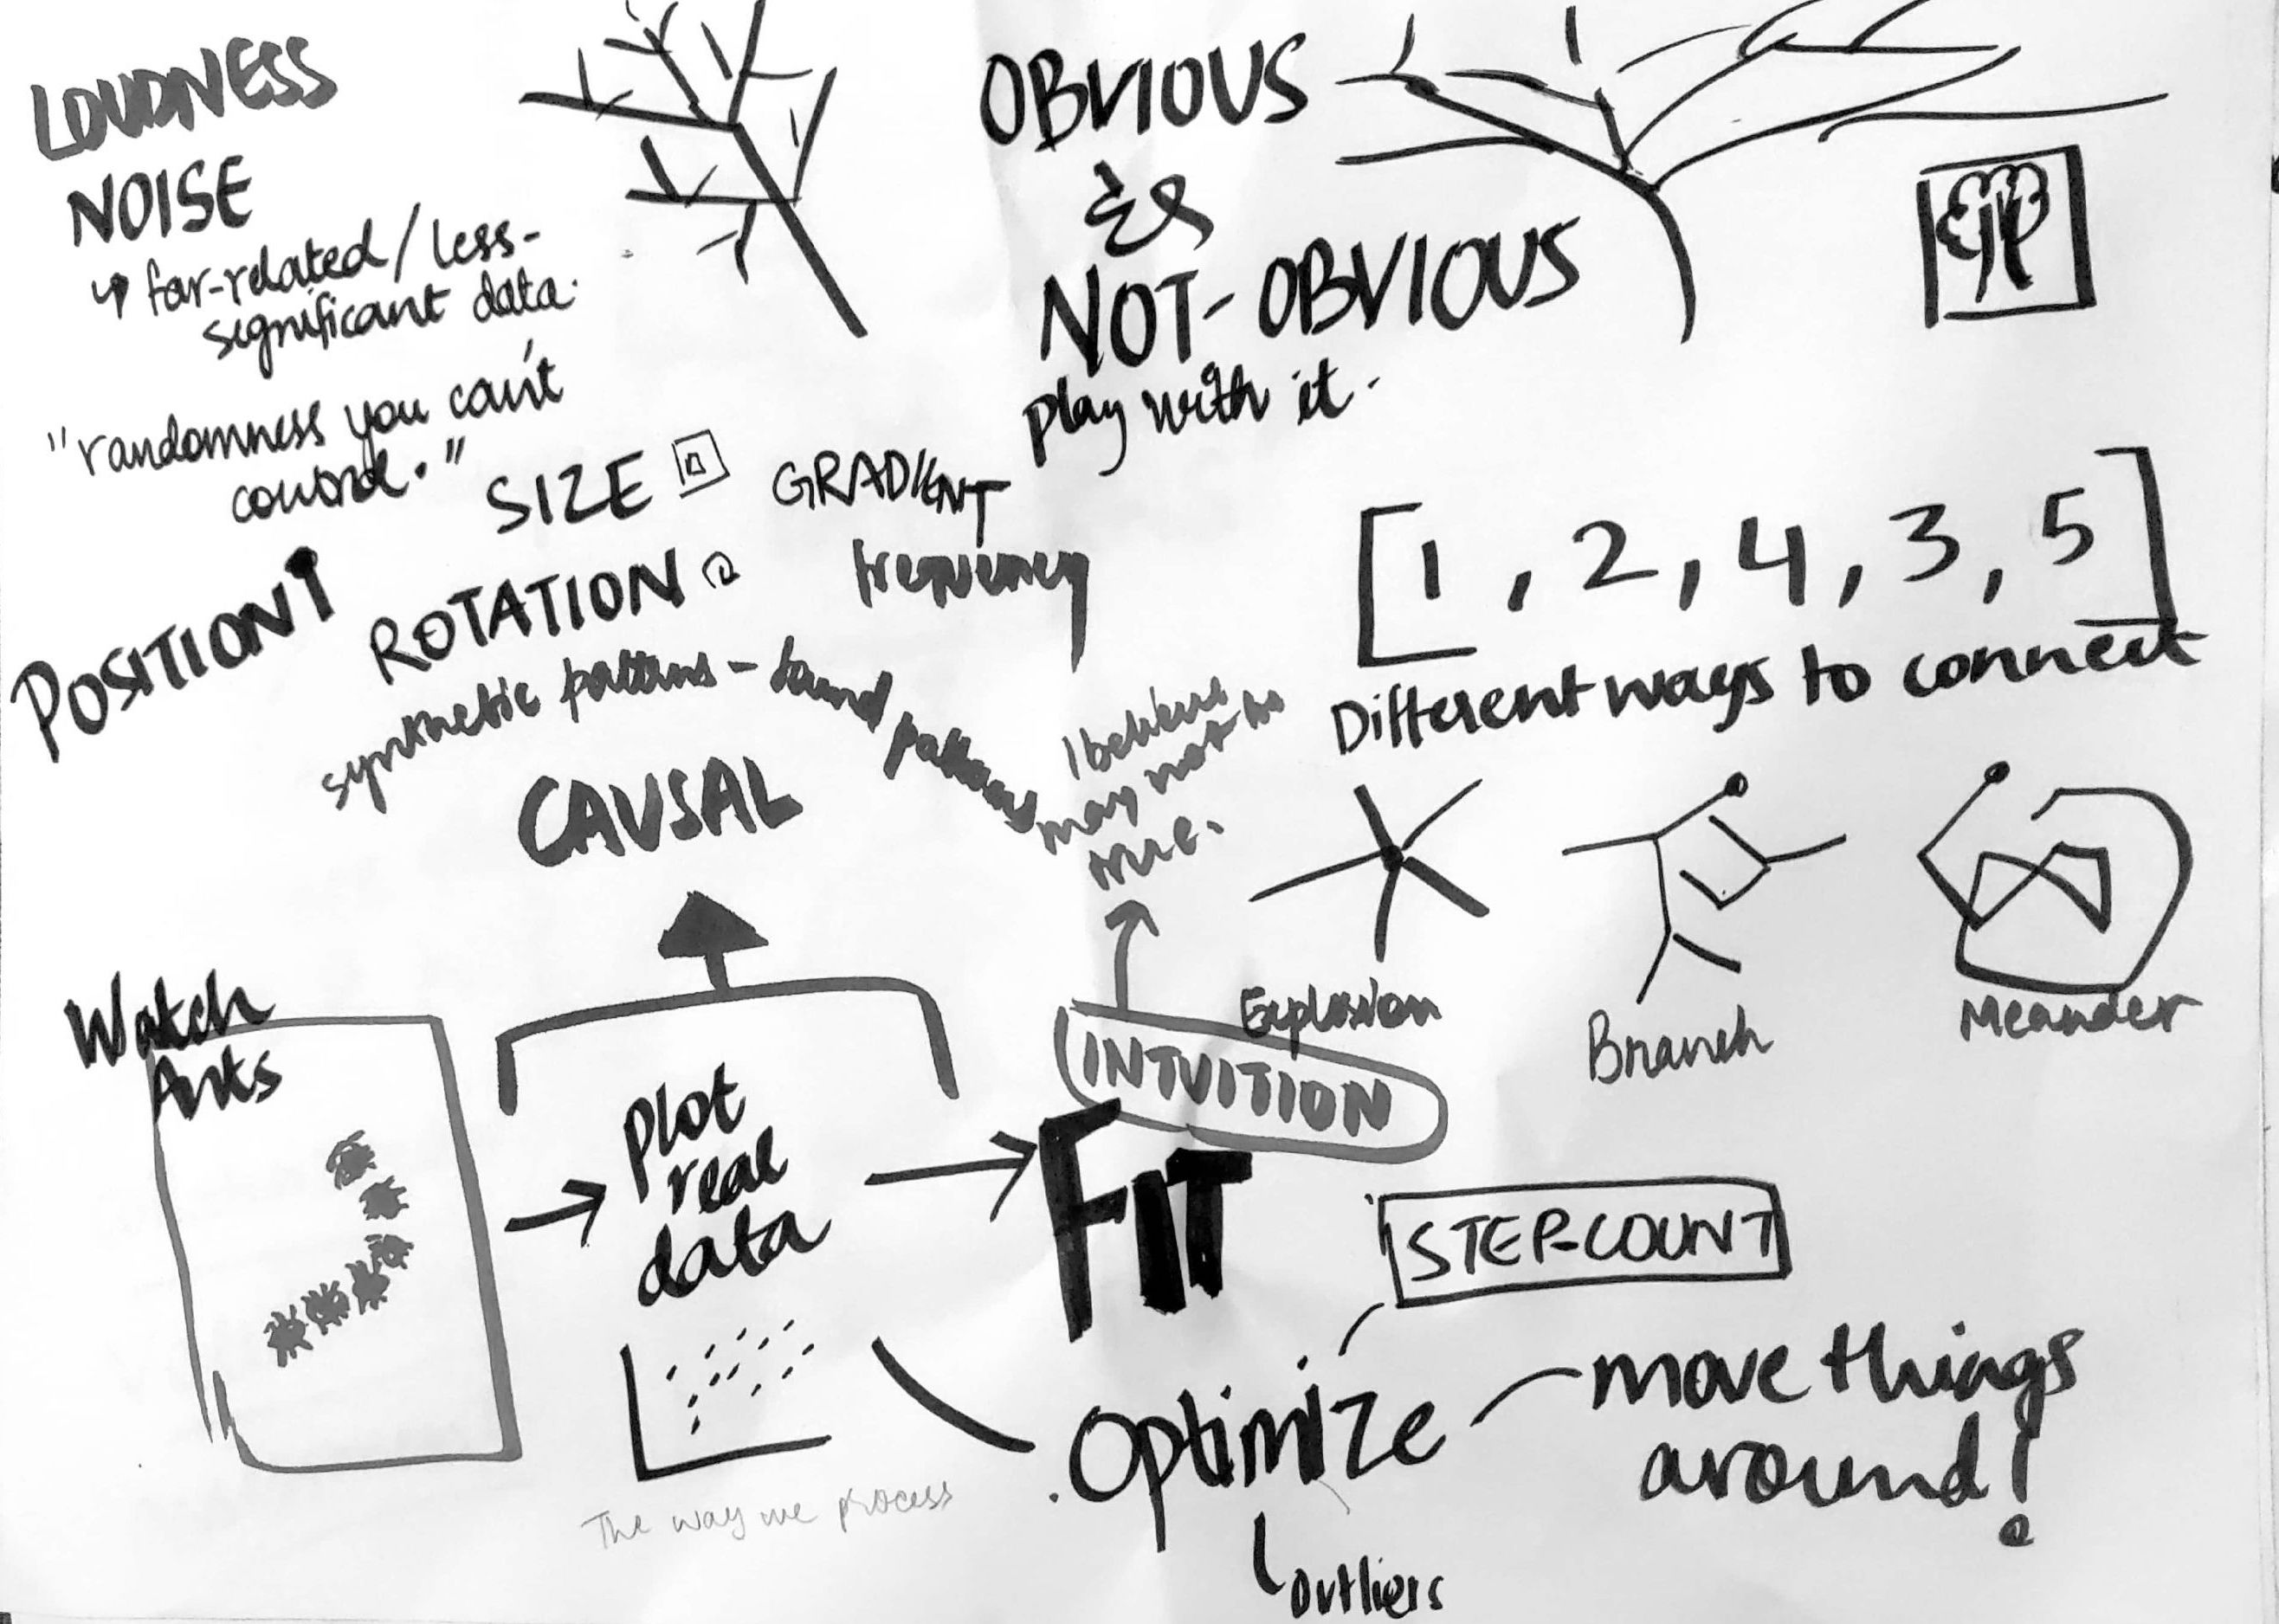
\includegraphics[height=0.2\textwidth]{block6-3.jpg}
  \caption{Visual notes categorising how learning can be constructed physically}
\end{figure}

Since theme/idea of the project has been discovered, the next phase may not be about questioning the need of such AI kit in the school, but about identifying what would be the first thing that should be given to the teachers to teach their students about AI.

With me so far? Glad you made it here. Now onto what’s next.

\begin{figure}[h]
  \center
  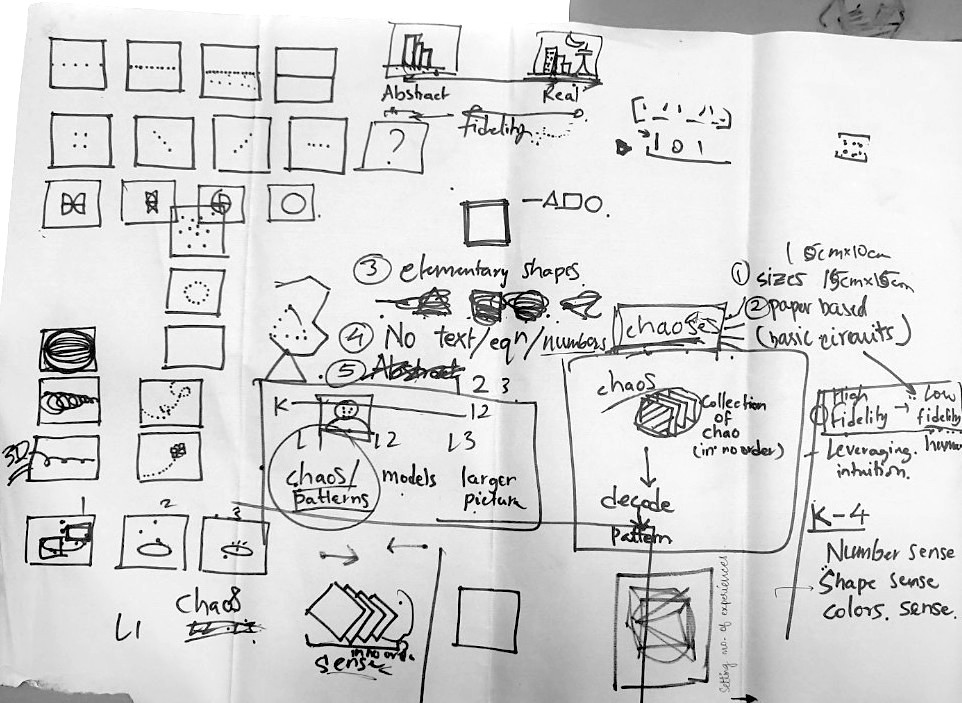
\includegraphics[height=0.3\textwidth]{block7-1.jpg}
  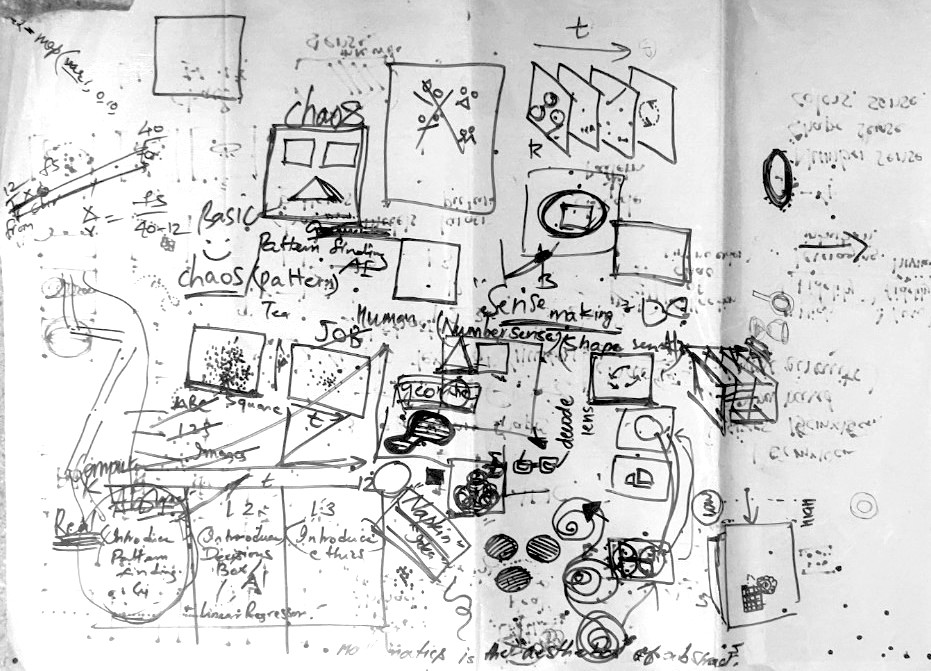
\includegraphics[height=0.3\textwidth]{block7-3.jpg}
  \caption{Planning the toolkit}
\end{figure}

Artificial Intelligence as a subject offers a vast variety of themes to be an anchor to introduce AI to a layman. For each to be the first thing that explains machine intelligence, an abstract introduction to the related processes felt complex for K-12. It was then understood that a toolkit, pertaining to developing age groups could be able to accommodate the goal of collective understanding and acceptance of different ways/possibilities of thinking and learning. Only by addressing how things relate and cause effects, we can conceptualise solutions for the upcoming ever-complex future.

Artificial Intelligence as a subject offers a vast variety of themes to be an anchor to introduce AI to a layman. For each to be the first thing that explains machine intelligence, an abstract introduction to the related processes felt complex for K-12. It was then understood that a toolkit, pertaining to developing age groups could be able to accommodate the goal of collective understanding and acceptance of different ways/possibilities of thinking and learning. Only by addressing how things relate and cause effects, we can conceptualise solutions for the upcoming ever-complex future.

\begin{figure}[h]
  \center
  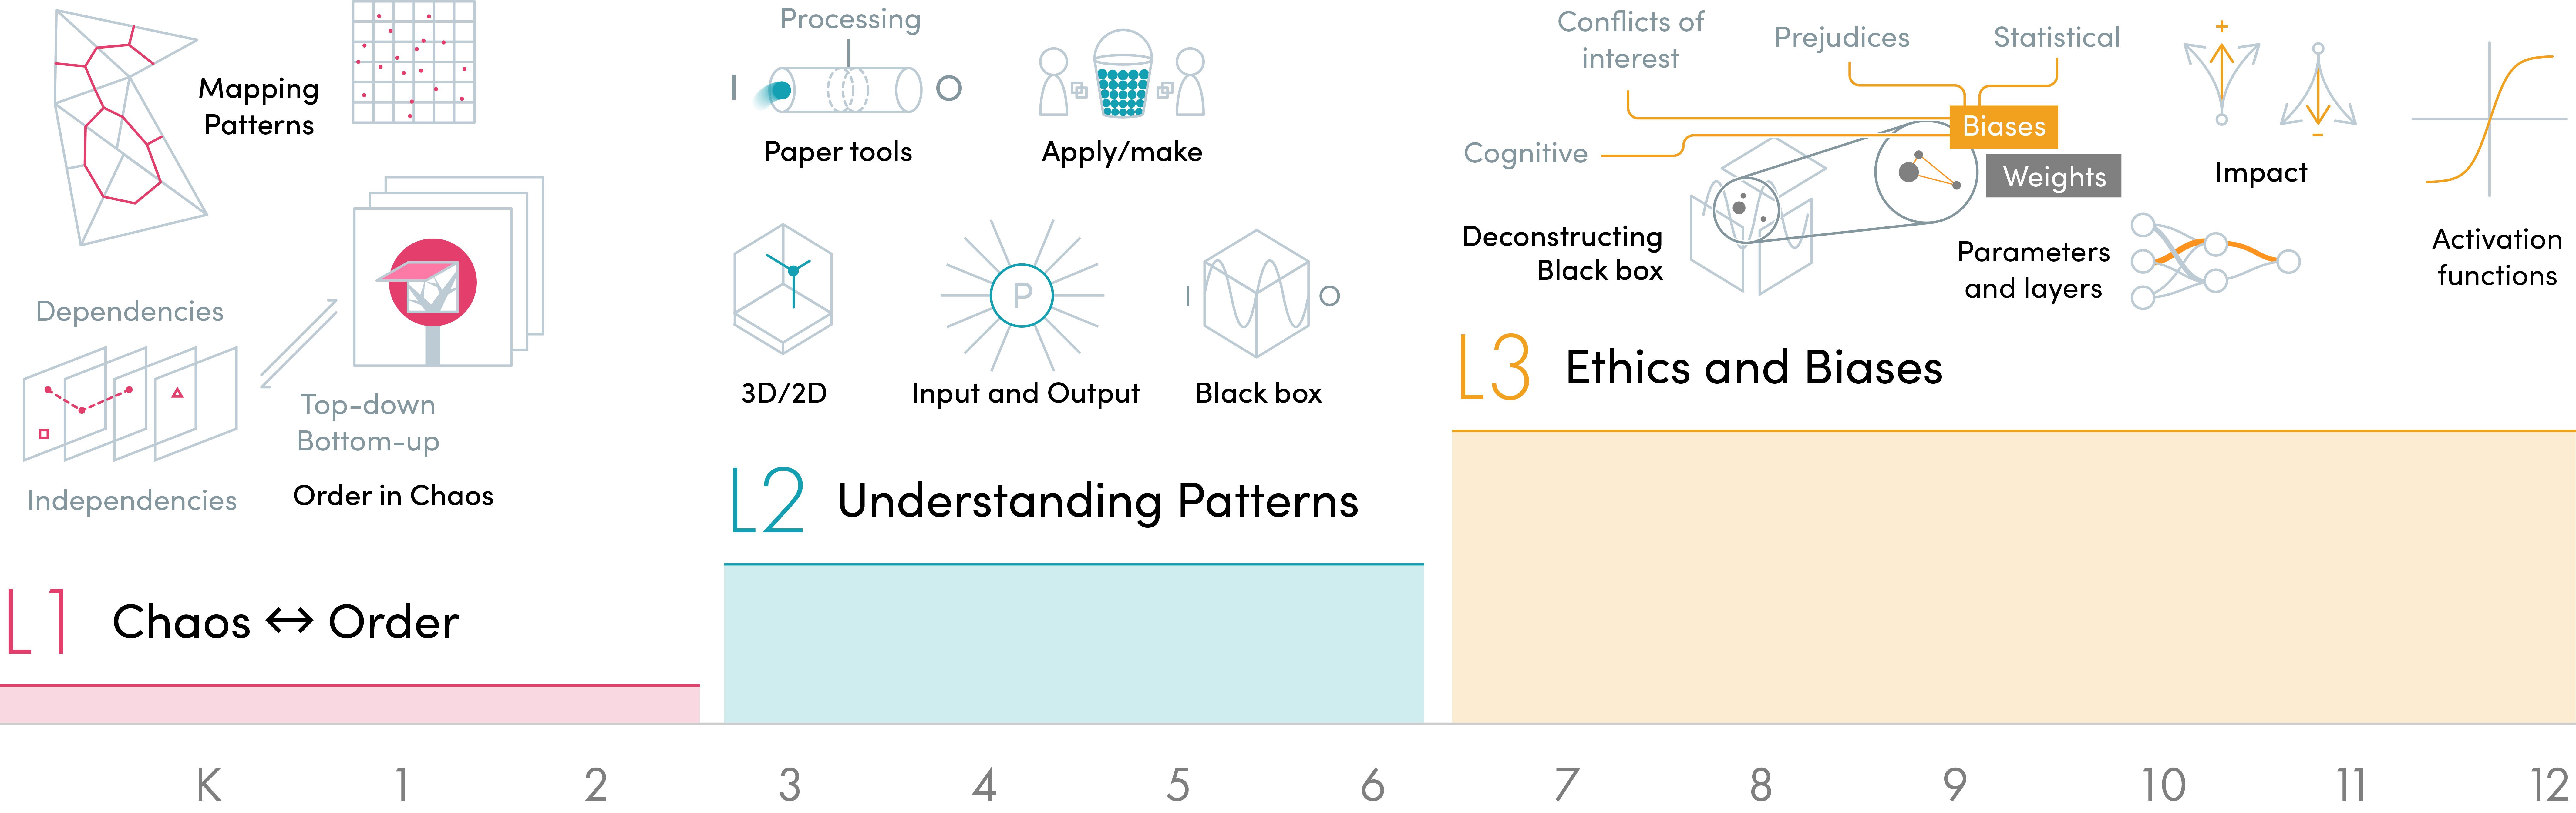
\includegraphics[width=\textwidth]{sigmoid_concept.png}
  \caption{Sigmoid Concept juxtaposed on K-12 curriculum}
\end{figure}

\bibliography{ref.bib}
\bibliographystyle{plain}

\vspace{1cm}
\textbf{About the author.} Simran Singh is a Human-Centered Design student pursuing her undergraduate degree at Srishti, Bangalore. An analytical-dreamer, her work focuses on understanding the use-cases of emerging technologies and applying it in a user-friendly context. She sees value in algorithmic thinking to help understand, decode and apply at the design context.

\vspace*{\fill}
\rule{\textwidth}{0.4pt}
\footnotesize \mscpy. All rights reserved. This paper or any portion thereof may not be reproduced or used in any manner whatsoever without the express written permission of Mathscapes and the author(s) of this paper except for the use of brief quotations in a review.

\end{document}
